\documentclass[sigconf,review,anonymous]{acmart}

\usepackage{listings}
\usepackage{subcaption}

\settopmatter{printacmref=false}

% names
\newcommand{\cfg}{\text{CFG}}
\newcommand{\bnf}{\text{BNF}}
\newcommand{\es}{\text{ES}}
\newcommand{\bnfes}{\bnf_\es}
\newcommand{\peg}{\text{PEG}}

% codes
\newcommand{\scode}[1]{\texttt{\scriptsize#1}}
\newcommand{\code}[1]{\texttt{\footnotesize#1}}
\newcommand{\kwtrue}{\code{true}}
\newcommand{\kwt}{\code{\#t}}
\newcommand{\kwfalse}{\code{false}}
\newcommand{\kwf}{\code{\#f}}

%BNF_ES
\newcommand{\symb}{s}
\newcommand{\NT}[1]{#1}
\newcommand{\T}[1]{\code{#1}}
\newcommand{\argument}{a}
\newcommand{\param}{p}
\newcommand{\butnot}{\!\smallsetminus\!}
\newcommand{\rhs}{\alpha}
\newcommand{\cond}{c}
\newcommand{\nolt}{\left<\neg\code{LT}\right>}

% colors
\newcommand{\inred}[1]{{\color{red}{#1}}}

% lookahead
\newcommand{\symbfirst}[1]{\textbf{first}_\symb(#1)}
\newcommand{\rhsfirst}[1]{\textbf{first}_\rhs(#1)}
\newcommand{\fail}{FAIL}
\newcommand{\emptyfirst}{\circ}
\newcommand{\firstplus}{:\!\!+\;}
\newcommand{\la}{L}
\newcommand{\getlap}[1]{\textbf{get}_\symb(#1)}

% IR_ES language
\newcommand{\ires}{\text{IR}_\text{ES}}
\newcommand{\tend}{\downarrow}
\newcommand{\tin}{\searrow}
\newcommand{\tout}{\swarrow}
\newcommand{\tstar}{\star}

% hint image
\newcommand{\hint}{%
  \begingroup\normalfont
  
\includegraphics[height=\fontcharht\font`\B]{img/hint.png}%
  \endgroup
}

% Our tool name
\newcommand{\tool}{\text{\sf JISET}}


\begin{document}

\title{$\bigtool$: JavaScript Specification Type Analyzer using Refinement}
% \title{$\bigtool$: ECMAScript Static Checker based on Refinement Types}

\author{Jihyeok Park}
\affiliation{%
  \institution{KASIT}
  \city{Daejeon}
  \country{South Korea}}
\email{jhpark0223@kaist.ac.kr}

\author{Seungmin An}
\affiliation{%
  \institution{KASIT}
  \city{Daejeon}
  \country{South Korea}}
\email{h2oche@kaist.ac.kr}

\author{Yusung Sim}
\affiliation{%
  \institution{KASIT}
  \city{Daejeon}
  \country{South Korea}}
\email{yusungsim@kaist.ac.kr}

\author{Wonho Shin}
\affiliation{%
  \institution{KASIT}
  \city{Daejeon}
  \country{South Korea}}
\email{new170527@kaist.ac.kr}

\author{Sukyoung Ryu}
\affiliation{%
  \institution{KASIT}
  \city{Daejeon}
  \country{South Korea}}
\email{sryu.cs@kaist.ac.kr}

\begin{abstract}
  JavaScript is one of mainstream programming languages for client-side
  programming, server-side programming, and even embedded systems.  Thus,
  various JavaScript engines are developed and maintained in diverse fields, and
  they must conform to the syntax and semantics described in ECMAScript, the
  standard specification of JavaScript.  Since an incorrect description in
  ECMAScript can lead to the wrong JavaScript engine implementations, checking
  the correctness of ECMAScript is essential.  However, all the specification
  updates are currently manually reviewed by the Ecma Technical Committee 39
  (TC39) without any automated tools.  Moreover, in late 2014, the committee
  announced yearly release cadence and open development process of ECMAScript to
  adapt to evolving development environments quickly.  Because of such frequent
  updates, checking the correctness of ECMAScript becomes more labor-intensive
  and error-prone.

  To alleviate the problem, we propose $\tool$, a JavaScript Specification Type
  Analyzer using Refinement.  It is the first tool that performs \textit{type
  analysis} on JavaScript specifications and detects specification bugs using a
  \textit{bug detector}.  For a given specification, $\tool$ first compiles each
  abstract algorithm written in a structured natural language to a corresponding
  function in $\ires$, an untyped intermediate representation for ECMAScript.
  Then, it performs type analysis for compiled functions with specification
  types defined in ECMAScript.  Based on the result of type analysis, $\tool$
  detects specification bugs using a bug detector consisting of four checkers.
  Moreover, to increase precision of type analysis, we present
  \textit{condition-based refinement} for type analysis, which prunes out
  infeasible abstract states using conditions of assertions and branches.  We
  evaluated $\tool$ with all 864 versions in the official ECMAScript repository
  for the recent three years from 2018 to 2021.  Our tool took \inred{230}
  seconds on average to perform type analysis for each version, and detected
  \inred{200} type-related specification bugs with \inred{50.3}\% precision;
  \inred{91} out of \inred{200} bugs are true bugs.  Among them, \inred{14} bugs
  are newly detected by $\tool$ and the committee confirmed all of them.
\end{abstract}


\keywords{JavaScript, mechanized specification, type analysis, refinement, bug
detection}

\maketitle

\section{Introduction}\label{sec:intro}

JavaScript is one of the most popular programming languages.  According to the
2020 State of the Octoverse\footnote{https://octoverse.github.com/}, which is
the annual report of GitHub, the most dominated programming language in GitHub
repositories was JavaScript since 2014 to 2020.  While JavaScript was initially
designed for client-side programming in web browsers, now it is widely used in
server-side programming~\cite{nodejs} and even in embedded
systems~\cite{espruino, tessel2, moddable}.  Thus, its engines are also
developed and maintained in diverse fields conforming to ECMAScript, the
JavaScript standard specification that describes the syntax and semantics of
JavaScript.

The correctness of ECMAScript becomes more important because an incorrect
description of syntax or semantics in the specification can lead to the wrong
implementation of existing JavaScript engines used in various fields.  However,
all the specification updates are currently manually checked by the Ecma
Technical Committee 39 (TC39) without any automated tools.  This manual checking
process is obviously labor-intensive and also error-prone thus the current
JavaScript specification is vulnerable to specification bugs.  Besides, in late
2014, the committee announced yearly release cadence and open development
process of ECMAScript to quickly adapt to an evolving development environment.
According to \citet{jiset}, the average number of updated steps of abstract
algorithms between consecutive releases from ES7 (2016) to ES10 (ES2019) is
9645.5.  In the official repository of ECMAScript, \inred{X,XXX} pull requests
and \inred{X,XXX} commits exist in the master branch.  Therefore, it makes more
difficult to manually check all the specification updates using limited human
resources.

% TODO: links in footnote
Unfortunately, there is no existing tool to automatically detect bugs in the
rapidly evolved JavaScript specifications.  Thus, the committee of ECMAScript
have tried to resolve this problem using additional annotations in abstract
algorithms.  Additional annotations make the specification more readable and
also they are useful for the specification-based tools such as JavaScript
engines~\cite{v8, graaljs, qjs, moddable}, debuggers~\cite{jsexplain}, static
analyzers~\cite{safe, tajs, jsai, wala}, and verification tools~\cite{javert}.
Thus, they decided to manually insert two different annotations: 1)
\textit{assertions} to denotes the assumptions in a certain point of abstract
algorithms, and 2) two different \textit{prefixes} $\code{?}$ and $\code{!}$ to
represent whether completion records might be abrupt or not.  For example,
``Assert: Type(\textit{O}) is Object'' denotes that the variable $\textit{O}$
always has an Object value at this point and ``? \textbf{GetV}(\textit{V},
\textit{P})'' denotes that return values of \textbf{GetV}(\textit{V},
\textit{P}) might be abrupt completions.  Moreover, they recently started the
internal discussion of manual type annotations for variables, parameters, and
return values for each abstract
algorithm~\footnote{https://github.com/tc39/ecma262/pull/545\#issuecomment-559292107}.
However, to manually annotate types for all of them without any automated tool
is also labor-intensive and error-prone.  Furthermore, even though the such
manual type annotations can give more information for manual checking of
specification updates, it still does not provide any automatic approach to
detect specification bugs.

To alleviate this problem, we propose a tool $\tool$, a \textbf{J}avaScript
\textbf{S}pecification \textbf{T}ype \textbf{A}nalyzer using
\textbf{R}efinement.  The main idea of our tool is to perform \textit{type
analysis} for JavaScript specifications to statically detect type-related
specification bugs in an automatic way.  However, it is difficult to directly
perform type analysis to ECMAScript because its abstract algorithms are written
in a natural language.  For a decade, researchers~\cite{lambdajs, jscert, kjs}
have tried to formally define various mechanized JavaScript specification for a
specific version of ECMAScript by hand.  However, the manual formalization is
not suitable for the automatic detection of bugs in the rapidly evolved
JavaScript specifications.  On the other hand, several approaches to utilize
information directly extracted from specifications written in a natural language
are recently presented in diverse fields such as system architectures~\cite{x86,
arm}, network protocols~\cite{basespec}, and language
specifications~\cite{spectest}.  For JavaScript, \citet{jiset} presents $\jiset$
that automatically compiles each abstract algorithm written in a structured
natural language to the corresponding function of $\ires$, an untyped
intermediate representation for ECMAScript.  Therefore, we utilize this tool to
automatically get mechanized specifications for JavaScript.

For the compiled mechanized specifications, $\tool$ performs type analysis for
compiled functions with specification types defined in ECMAScript.  ECMAScript
contains not only JavaScript language types but also specification types such as
abstract syntax trees (ASTs), internal records (i.e. environments, completions,
or property descriptors), and internal list-like structures.  Our tool extract
syntax and table-based type information from ECMAScript and constructs type
hierarchy and fields for ASTs and records.  Based on the extracted types,
$\tool$ performs type analysis and detects specification bugs using a
\textit{bug detector} consisting of four different checkers: 1) reference
checker, 2) arity checker, 3) assertion checker, and 4) operand checker.
Moreover, to increase precision of type analysis, we also present
\textit{condition-based refinement} for type analysis on ECMAScript. Its main
concept is to prunes out infeasible abstract states by using conditions of
assertions and branches.  The refinement technique can reduce false alarms
caused by spurious types inferred by imprecise analysis.  We evaluate our tool
with all \inred{XXX} different versions existed in the official ECMAScript
repository for the recent \inred{three years from 2018 to 2021}.

In summary, our main contributions are as follows:
\begin{itemize}
  \item We present $\tool$, which is the first tool that performs \textit{type
    analysis} on ECMAScript to check the the correctness of JavaScript language
    specifications.  $\tool$ automatically detects specification bugs via the
    \textit{bug detector} consisting of four different checkers: 1) reference
    checker, 2) arity checker, 3) assertion checker, and 4) operand checker.
  \item We present \textit{condition-based refinement} for type analysis of
    ECMAScript to reduce false alarms by increasing the analysis precision.  Its
    main idea is to prune out infeasible abstract states by using conditions of
    assertions and branches.
  \item We demonstrate the practicality of $\tool$. For recent \inred{XXX}
    different versions of ECMAScript, our tool detected \inred{XXX}
    specification bugs including only \inred{XXX} false alarms caused by the
    imprecision of type analysis in \inred{XX} minutes on average.  Among
    \inred{XXX} true alarms, \inred{XXX} bugs are resolved after existing for
    \inred{XXX} days on average and \inred{XX} bugs still exist in the latest
    version of ECMAScript for \inred{XXX} days.  We reported all \inred{XX}
    newly found bugs and they are confirmed by the committee.
\end{itemize}

\section{Overview}\label{sec:overview}

\begin{figure}
  \centering
  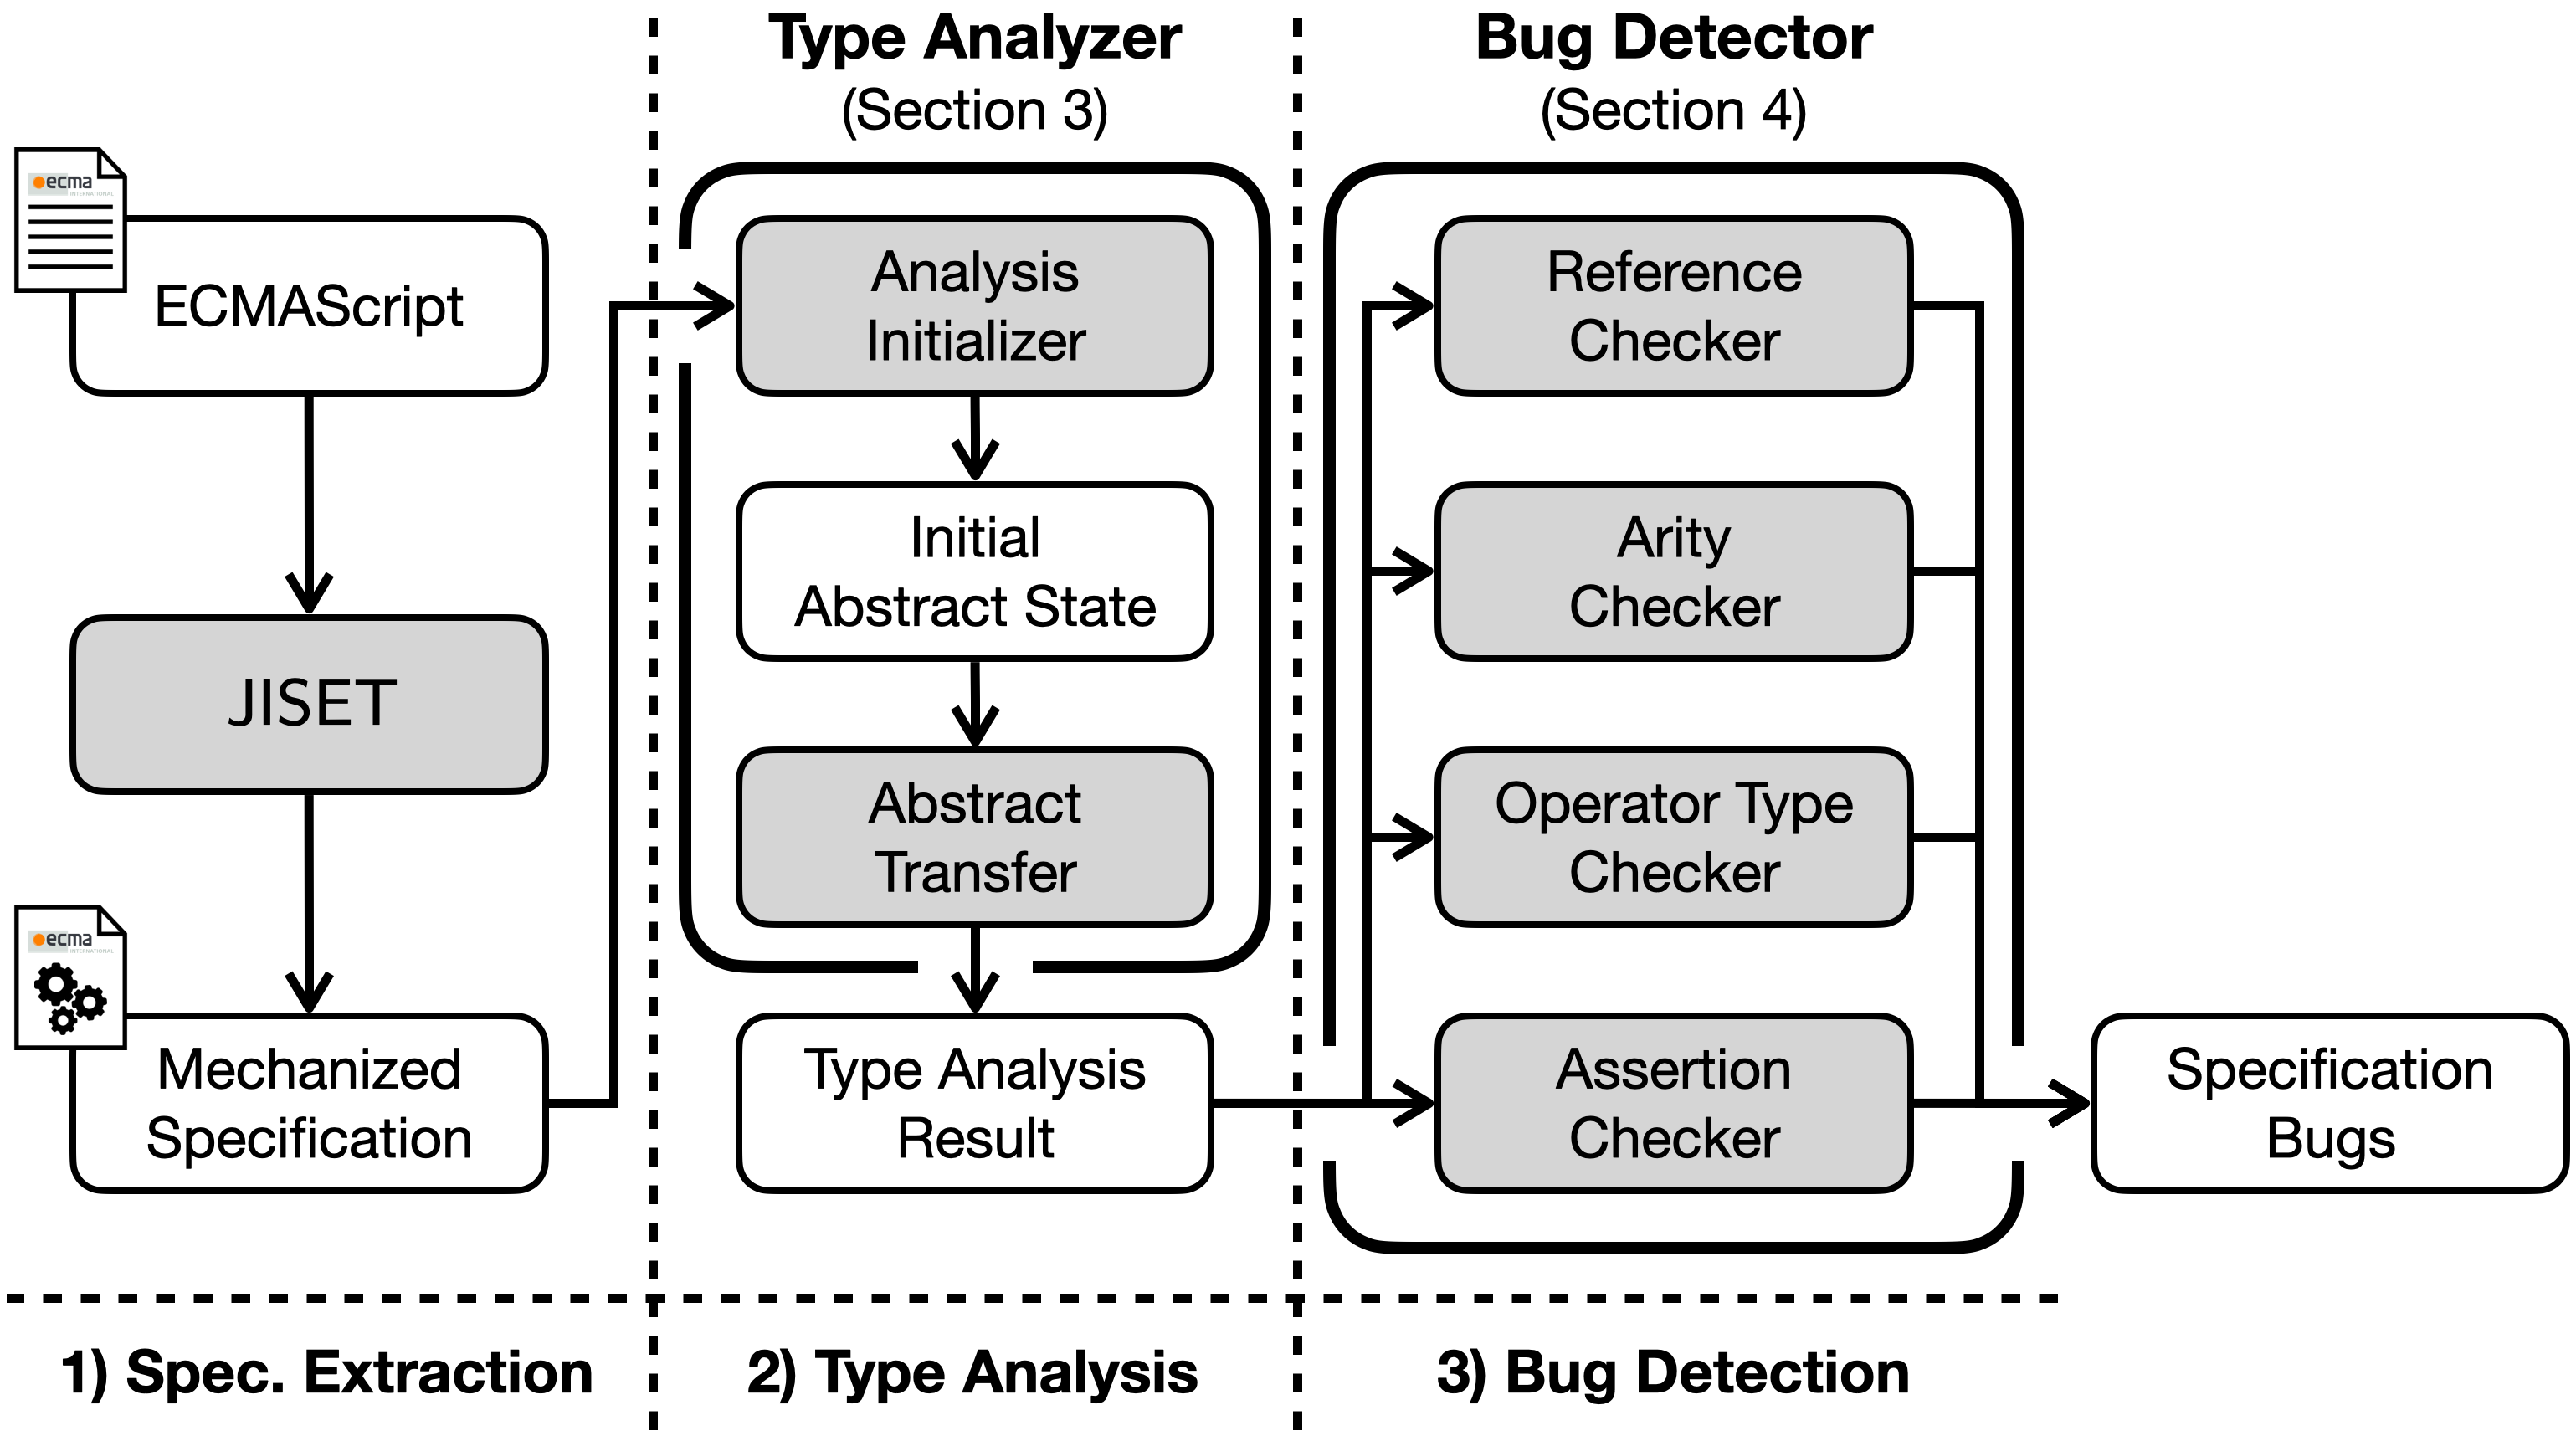
\includegraphics[width=\columnwidth]{img/overall}
  \caption{$\tool$: a type analyzer and a bug detector for
  mechanized specifications extracted from ECMAScript by $\jiset$}
  \label{fig:overall}
  \vspace*{-1.5em}
\end{figure}

\begin{figure*}[t]
  \centering
  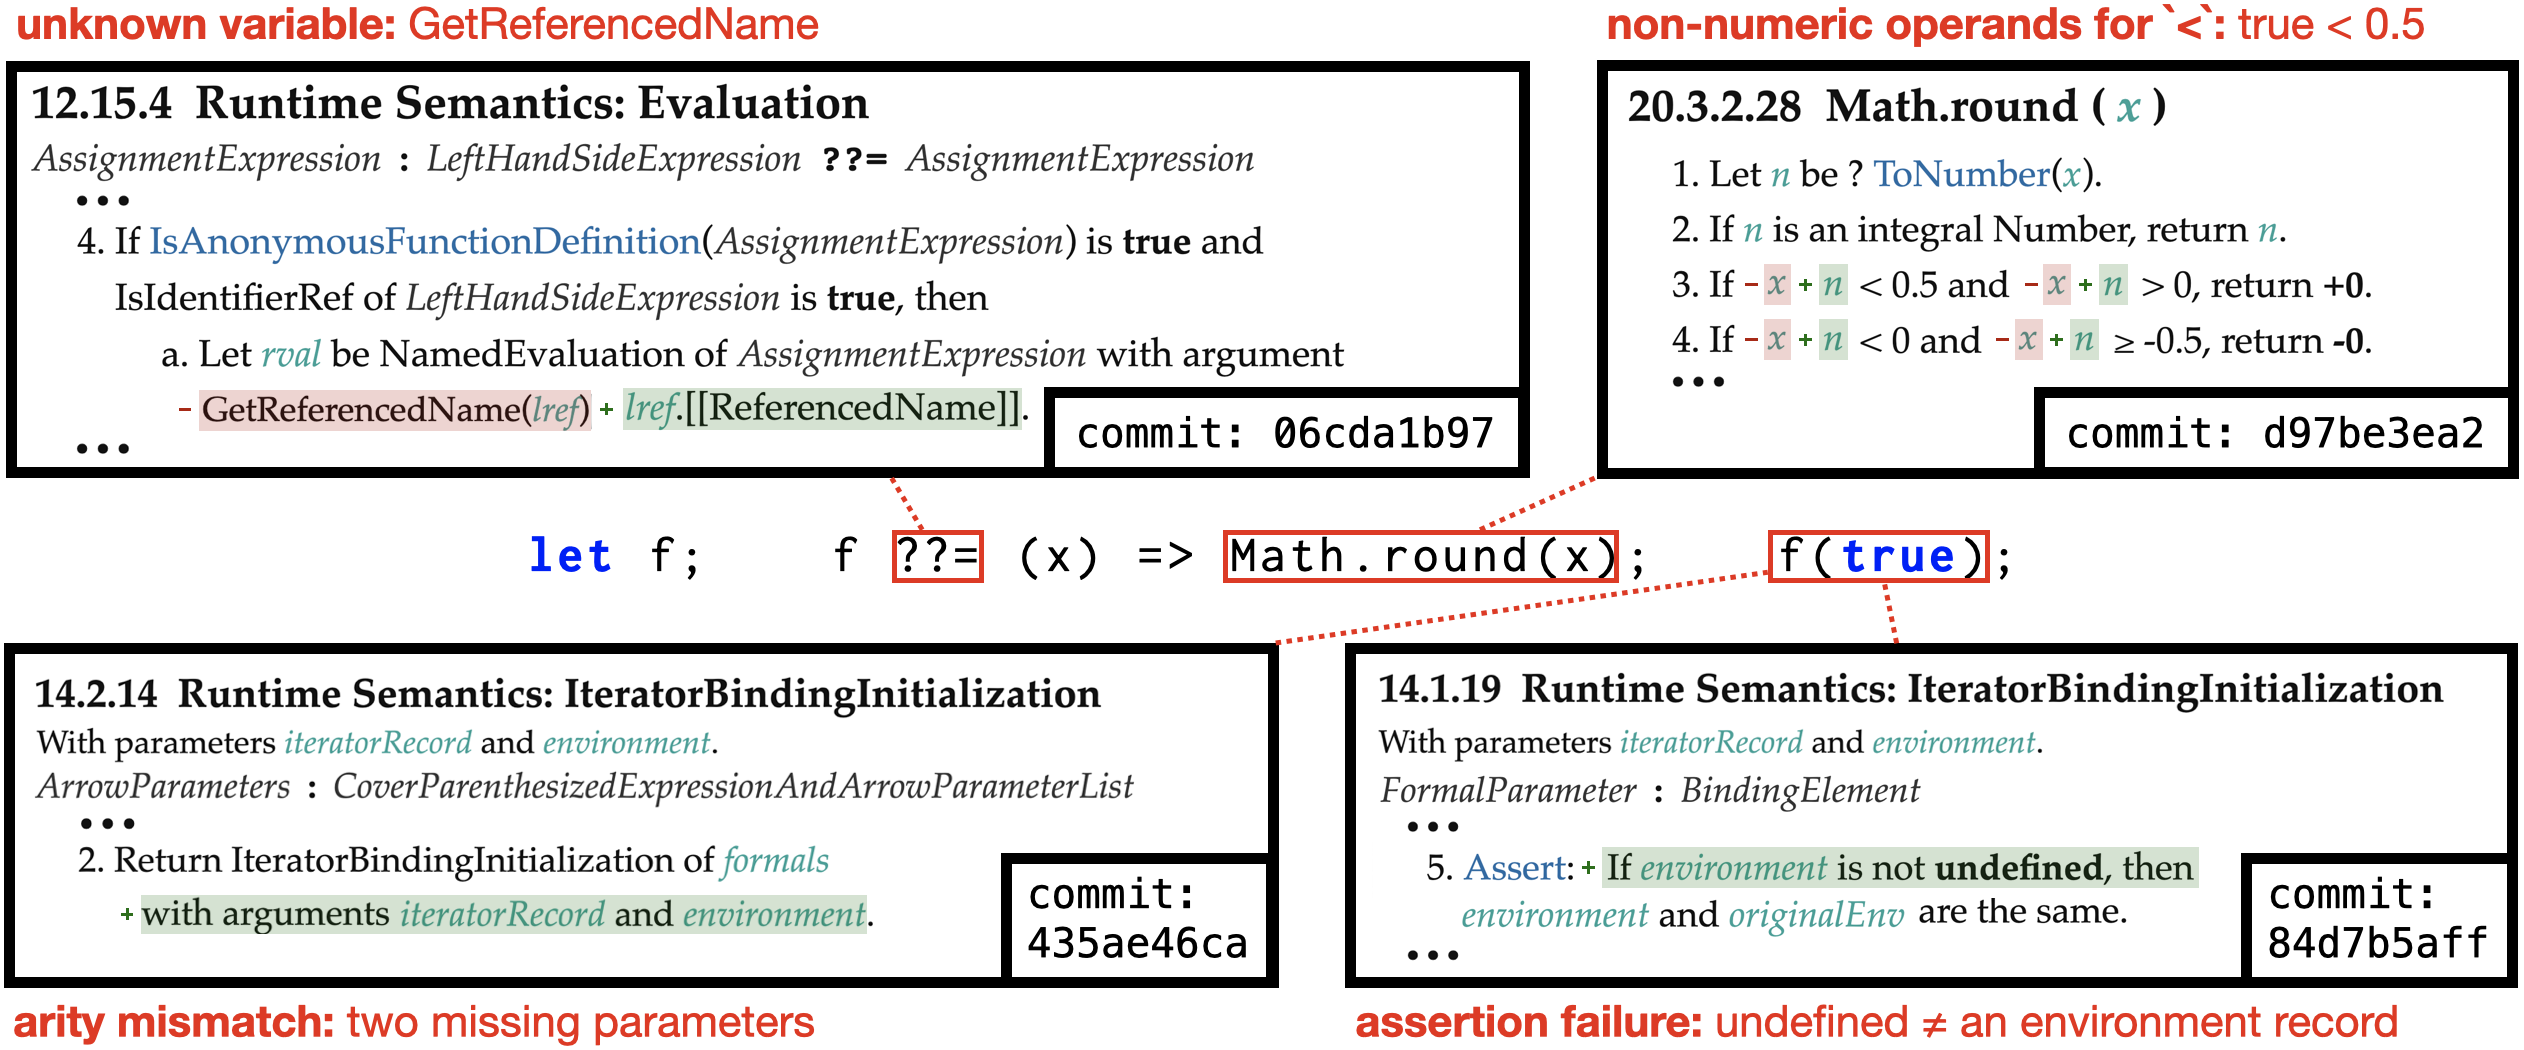
\includegraphics[width=.9\textwidth]{img/example}
%  \vspace*{-1.5em}
  \caption{An example JavaScript program with related previous specification
  bugs and their bug fixes}
  \label{fig:example}
  \vspace*{-1.5em}
\end{figure*}
% XXX
% \begin{lstlisting}[style=FigureJS]
% let f;    f ??= (x) => Math.round(x);    f(true);
% \end{lstlisting}

In this section, we demonstrate the overall structure of $\tool$ depicted in
Figure~\ref{fig:overall}.  It consists of three components:
1) specification extraction, 2) type analysis, and 3) bug detection.


\subsection{Specification Extraction}\label{sec:overview-spec-extract}
$\tool$ extracts the JavaScript syntax and semantics using $\jiset$
and extracts specification types from ECMAScript.

\paragraph{Syntax and Semantics}
ECMAScript describes the JavaScript syntax in an EBNF notation
and the semantics using abstract algorithms written in a structured natural language.
From ECMAScript, $\jiset$ synthesizes AST structures for syntax and 
compiles the abstract algorithms to $\ires$ functions with parameters
and local variables for semantics.  For example, the algorithm step
``\raisebox{-0.55ex}{
\includegraphics[width=0.55\columnwidth]{img/compile-example}}''
is compiled to an $\ires$ instruction $\kwlet \; \code{baseObj}\; \code{=}
\escaped\!  \code{ToObject(V.Base)}$.  To make it suitable for type analysis,
we modify $\ires$ as formally defined in Section~\ref{sec:ires}.

\paragraph{Types}
In addition to JavaScript types,
$\tool$ represents three kinds of specification types.
First, because ASTs are values in abstract algorithms, 
they can be stored in variables and passed as function arguments.
For ASTs, we use their production names as their
types and automatically link their corresponding syntax-directed algorithms to their fields.
Second, ECMAScript supports various record types and fields
whose possible values are defined in their corresponding tables.
For example, ``Table 9: Completion Record Fields'' in the latest
ECMAScript describes the fields of the completion records.
% The newest version contains tens of tables for record types, and they are backward compatible in general.
Thus, we manually model the fields of record types based on the tables
in the latest version and use them in a type analysis.
Third, for list-like structures, we define the empty list type
$\clist{}$ and parametric list types $\clist{\tau}$.

\subsection{Type Analysis}\label{sec:overview-type-analysis}

$\tool$ performs a type analysis with flow-sensitivity and
type-sensitivity for arguments.
Each function is split into multiple flow- and type-sensitive views, and an
abstract state stores mapping from views to corresponding abstract environments.
To handle views separately, we use a worklist algorithm.
The type analyzer consists of two sub-modules: an \textit{analysis initializer} and an
\textit{abstract transfer function}.

\paragraph{Analysis Initializer} It defines the initial abstract state and the
initial set of views for a worklist. ECMAScript provides three
kinds of abstract algorithms: \textit{normal}, \textit{syntax-directed}, and \textit{built-in}. 
As for entry points of type analysis, we use syntax-directed algorithms and built-in algorithms
because they have their parameter types.  For each entry point, the
initializer defines its abstract environment with parameter types and adds the
flow- and type-sensitive views of the entry point to the worklist.

\paragraph{Abstract Transfer Function} For each iteration, the abstract transfer function gets a
specific view from the worklist and updates the abstract environments of the next
views based on the abstract semantics.  It adds the next views to the worklist if
it changes their abstract environments, and the iteration finishes when
the worklist becomes empty.  To increase the analysis precision, we
perform a condition-based refinement for an abstract environment when the current
control point is a branch or an assertion as described in Section~\ref{sec:refine}.

\subsection{Bug Detection}\label{sec:overview-bug-detect}

To detect specification bugs utilizing the type analysis, we develop
four checkers in a bug detector.  We explain the targets of the checkers
with an example JavaScript program that contains related previous specification bugs and
their bug fixes, as shown in Figure~\ref{fig:example}.

\paragraph{Reference Checker} The example JavaScript program first defines a
variable \jscode{f} without initialization, which has the value \jscode{undefined}.
It then assigns an anonymous function to \jscode{f} using the operator \jscode{??=}.
While the corresponding \textbf{Evaluation} algorithm in Figure~\ref{fig:example}(a) originally
used the \textbf{GetReferencedName} algorithm to get a reference name on line 4.a,
a contributor removed the \textbf{GetReferencedName} algorithm and replaced all its
invocations with accesses of the field [[ReferencedName]] on October 28, 2020.
However, the contributor missed several cases including the semantics of
\jscode{??=}, which was fixed by another contributor on November 3, 2020.
Thus, the unknown variable bug for \textbf{GetReferencedName} lasted for 7 days,
which the reference checker can detect.

\paragraph{Arity Checker} The program finally calls \jscode{f} with an argument \jscode{true}.
During the initialization of the function call, \textbf{IteratorBindingInitialization}
in Figure~\ref{fig:example}(b) is executed with additional parameters \textit{iteratorRecord} and
\textit{environment} to assign argument values to parameters.
However, a contributor missed passing additional arguments to them on line 2 in
\textbf{IteratorBindingInitialization} of \textit{ArrowParameters} on September 6, 2018.
It caused an arity mismatch bug, which lasted for 533 days until another
contributor fixed it on February 20, 2020. The arity checker can detect such arity mismatches.

\paragraph{Assertion Checker} During the initialization of the function call,
\textbf{IteratorBindingInitialization} of \textit{FormalParameter} in Figure~\ref{fig:example}(c)
contains another bug.
Even though the additional \textit{environment} parameter may contain \jscode{undefined},
a contributor did not consider it on line 5 in the initial commit of the open development process
on September 22, 2015.  It caused an assertion failure bug, which lasted for 1,297 days until another
contributor fixed it on April 10, 2019.
The assertion checker can detect such assertion failures.


\paragraph{Operand Checker} After the function call initialization, the
parameter \jscode{x} has the value \jscode{true}, and \jscode{Math.round} in Figure~\ref{fig:example}(d) is invoked
with the argument \jscode{true}.  The \jscode{Math.round} built-in library first
converts the given parameter \textit{x} to its corresponding number value
\textit{n} using \textbf{ToNumber}, and performs the remaining
steps using \textit{n}.  However, a contributor mistakenly used
\textit{x} instead of \textit{n} on lines 3 and 4 on September 11, 2020.
This bug caused the algorithm to compare the boolean value \jscode{true} with the
numeric value 0.5 or 0 in the example code.
This bug lived for two days until another contributor fixed it, and
the operand checker can detect them.

In the remainder of this paper, we explain the details of how to perform type
analysis for $\ires$ functions and how to increase the analysis precision using
the condition-based refinement (Section~\ref{sec:analyzer}) and how to detect
type-related specification bugs (Section~\ref{sec:checker}).  After we evaluate $\tool$
(Section~\ref{sec:eval}), we discuss related work (Section~\ref{sec:related})
and conclude (Section~\ref{sec:conclusion}).

\section{Type Analyzer}\label{sec:analyzer}

In this section, we explain the detail of the type analyzer of $\tool$. We first
formally define a modified $\ires$ and explain how to perform type analysis for
the modified $\ires$.  Moreover, we also explain a condition-based refinement of
type analysis based on conditions of assertions and branches to increase
analysis precision.

\subsection{Intermediate Representation}\label{sec:ires}

\begin{figure}
  \centering
  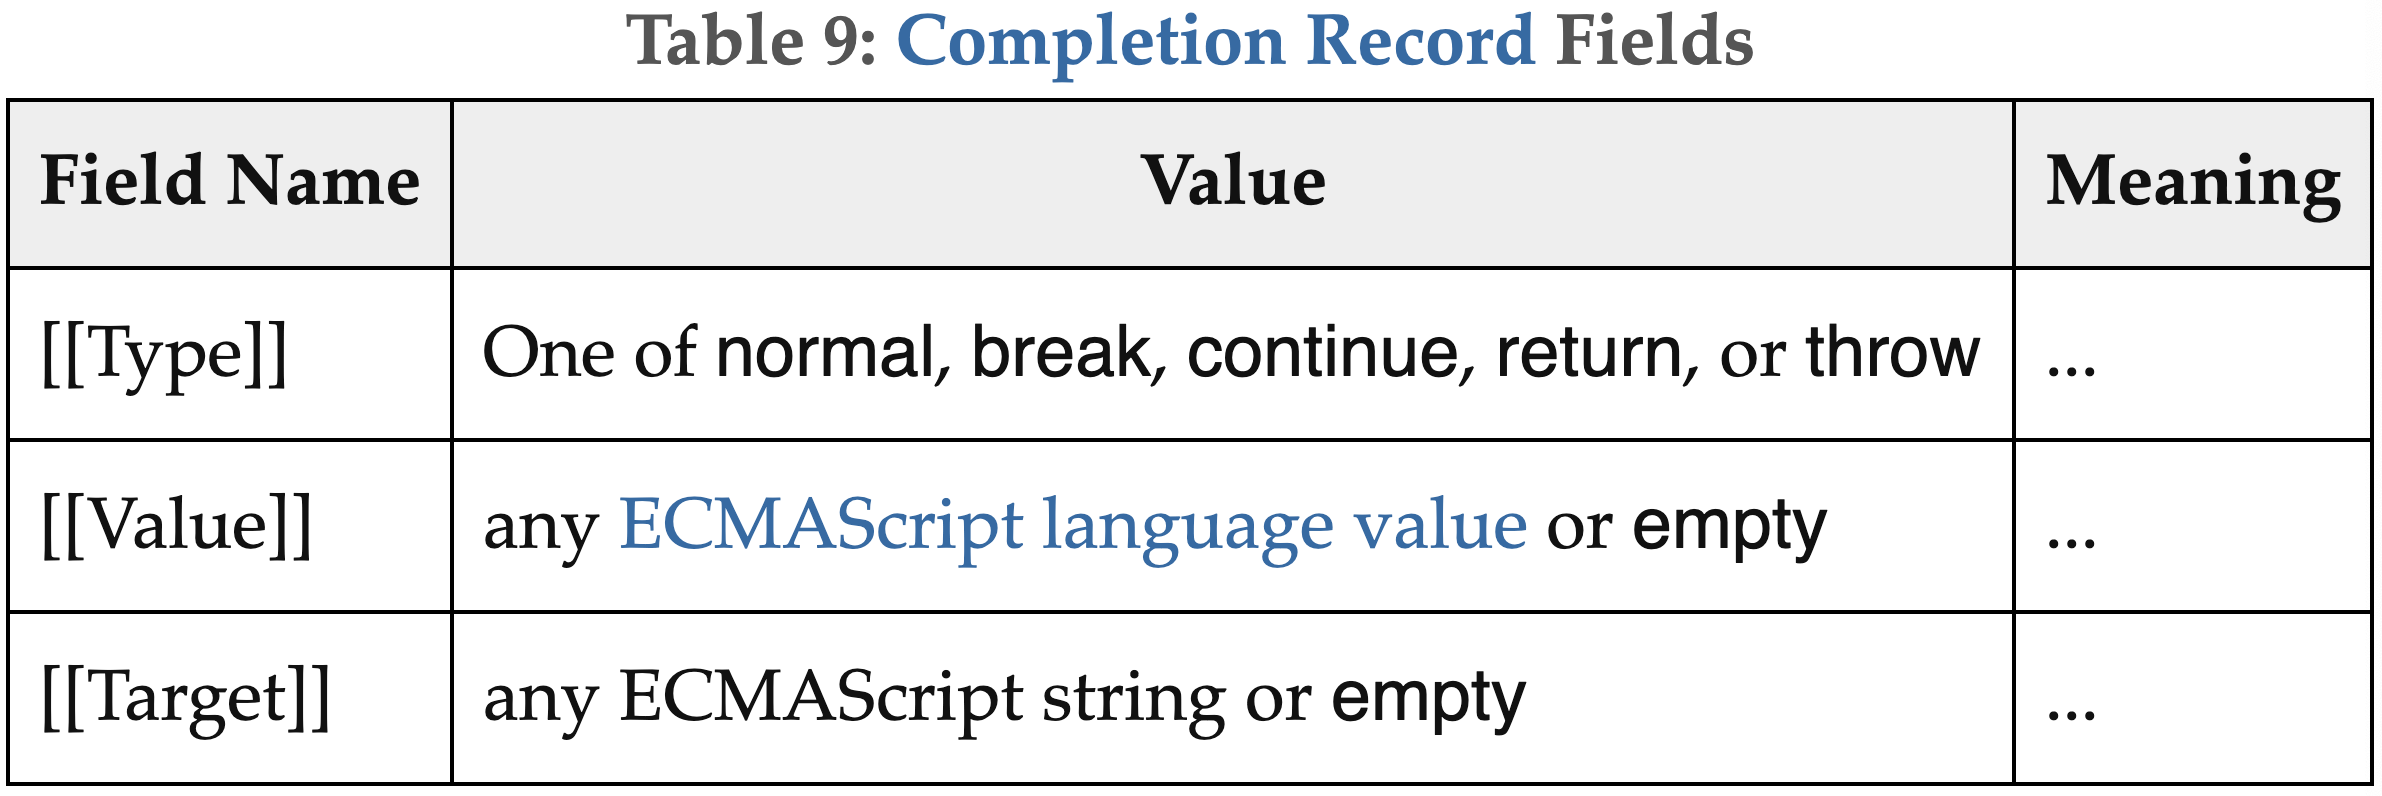
\includegraphics[width=0.48\textwidth]{img/record-fields-table}
  \vspace*{-1.5em}
  \caption{Fields of completion records in ES11.}
  \label{fig:record-fields-table}
  \vspace*{-1.5em}
\end{figure}

$\ires$ is an untyped intermediate representation introduced by \citet{jiset}.
To make it more suitable for type analysis, we modify it as a label-based
language as follows:
\small
\[
  \begin{array}{l@{~}r@{~}c@{~}r@{~}r@{~}l}
    \text{Functions}
    &\funcset&\ni&\func&::=&\kwdef \; \x (\x^*, \kwsl \x^* \kwsr). \; \lab\\

    \text{Instructions}
    &\instset&\ni&\inst&::=&
    \kwlet \; \x = \expr \mid
    \x = \kwrl \expr \; \expr^* \kwrr \mid
    \kwassert \; \expr \\

    &&&&\mid&
    \kwif \; \expr \; \lab \; \lab \mid
    \kwreturn \; \expr \mid
    \refer = \expr \\

    \text{References}
    &&&\refer&::=&
    \x \mid
    \refer \kwsl \expr \kwsr \\

    \text{Expressions}
    &&&\expr&::=&
    \tname \; \kwcl [\x: \expr]^* \kwcr \mid
    \clist{\expr^*} \mid
    \expr: \ty \mid
    \refer \kwexists \\

    &&&&\mid&
    \expr \bop \expr \mid
    \uop \; \expr \mid
    \refer \mid
    \const \mid
    \prim \\

    \text{Primitives}
    &\primset&\ni&\prim&::=&
    \undefval \mid \nullval \mid \bool \mid
    \num \mid \bigint \mid \str \mid \symb \\

    \text{Types}
    &\tyset&\ni&\ty&::=&\tname \mid \clist{} \mid \clist{\ty} \mid \tjs \mid
    \tprim \mid \undefval \mid \nullval\\

    &&&&\mid&
    \tbool \mid \tnumeric \mid \tnum \mid \tbigint \mid \tstr \mid \tsymb \\
  \end{array}
\]

A modified $\ires$ program $\prog = (\getfunc, \getinst, \getnext)$ is consists
of three mappings from labels;  $\getfunc: \labset \rightarrow \funcset$
represents that labels are in which functions, $\getinst: \labset \rightarrow
\instset$ represents instructions attached to labels, and $\getnext: \labset
\rightarrow \labset$ denotes next labels where a label $\lab \in \labset$
denotes a program point.  function $\kwdef \; \f (\x^*, \kwsl \y^* \kwsr). \;
\lab \in \funcset$ consists of its name $\f$, normal parameters $\x^*$, optional
parameters $\y^*$, and a body label $\lab$.  Although global variables exist in
ECMAScript, we assume that only local variables exist in this paper for brevity
An instruction $\inst$ is a variable declaration, a function call, an assertion,
a branch, a return, or an reference update.  Each invocation of an abstract
algorithm in ECMAScript is compiled to a function call instruction with a newly
introduced temporal variable.  We represent loops using branch instructions with
cyclic pointing of labels in the next mapping $\getnext$.  A reference $\refer$
is a variable $\x$ or a field access $\refer \kwsl \expr \kwsr$.  We use the
notation $\refer.\f$ to briefly represent $\refer \kwsl \code{"f"} \kwsr$. An
expression $\expr$ is a record, a list, a type check, an existence check, a
binary operation, a unary operation, a reference, a constant, or a primitive,
which is either $\undefval$, $\nullval$, a Boolean $\bool$, a Number $\num$, a
BigInt $\bigint$, a String $\str$, or a Symbol $\symb$.

\begin{figure}
  \centering
  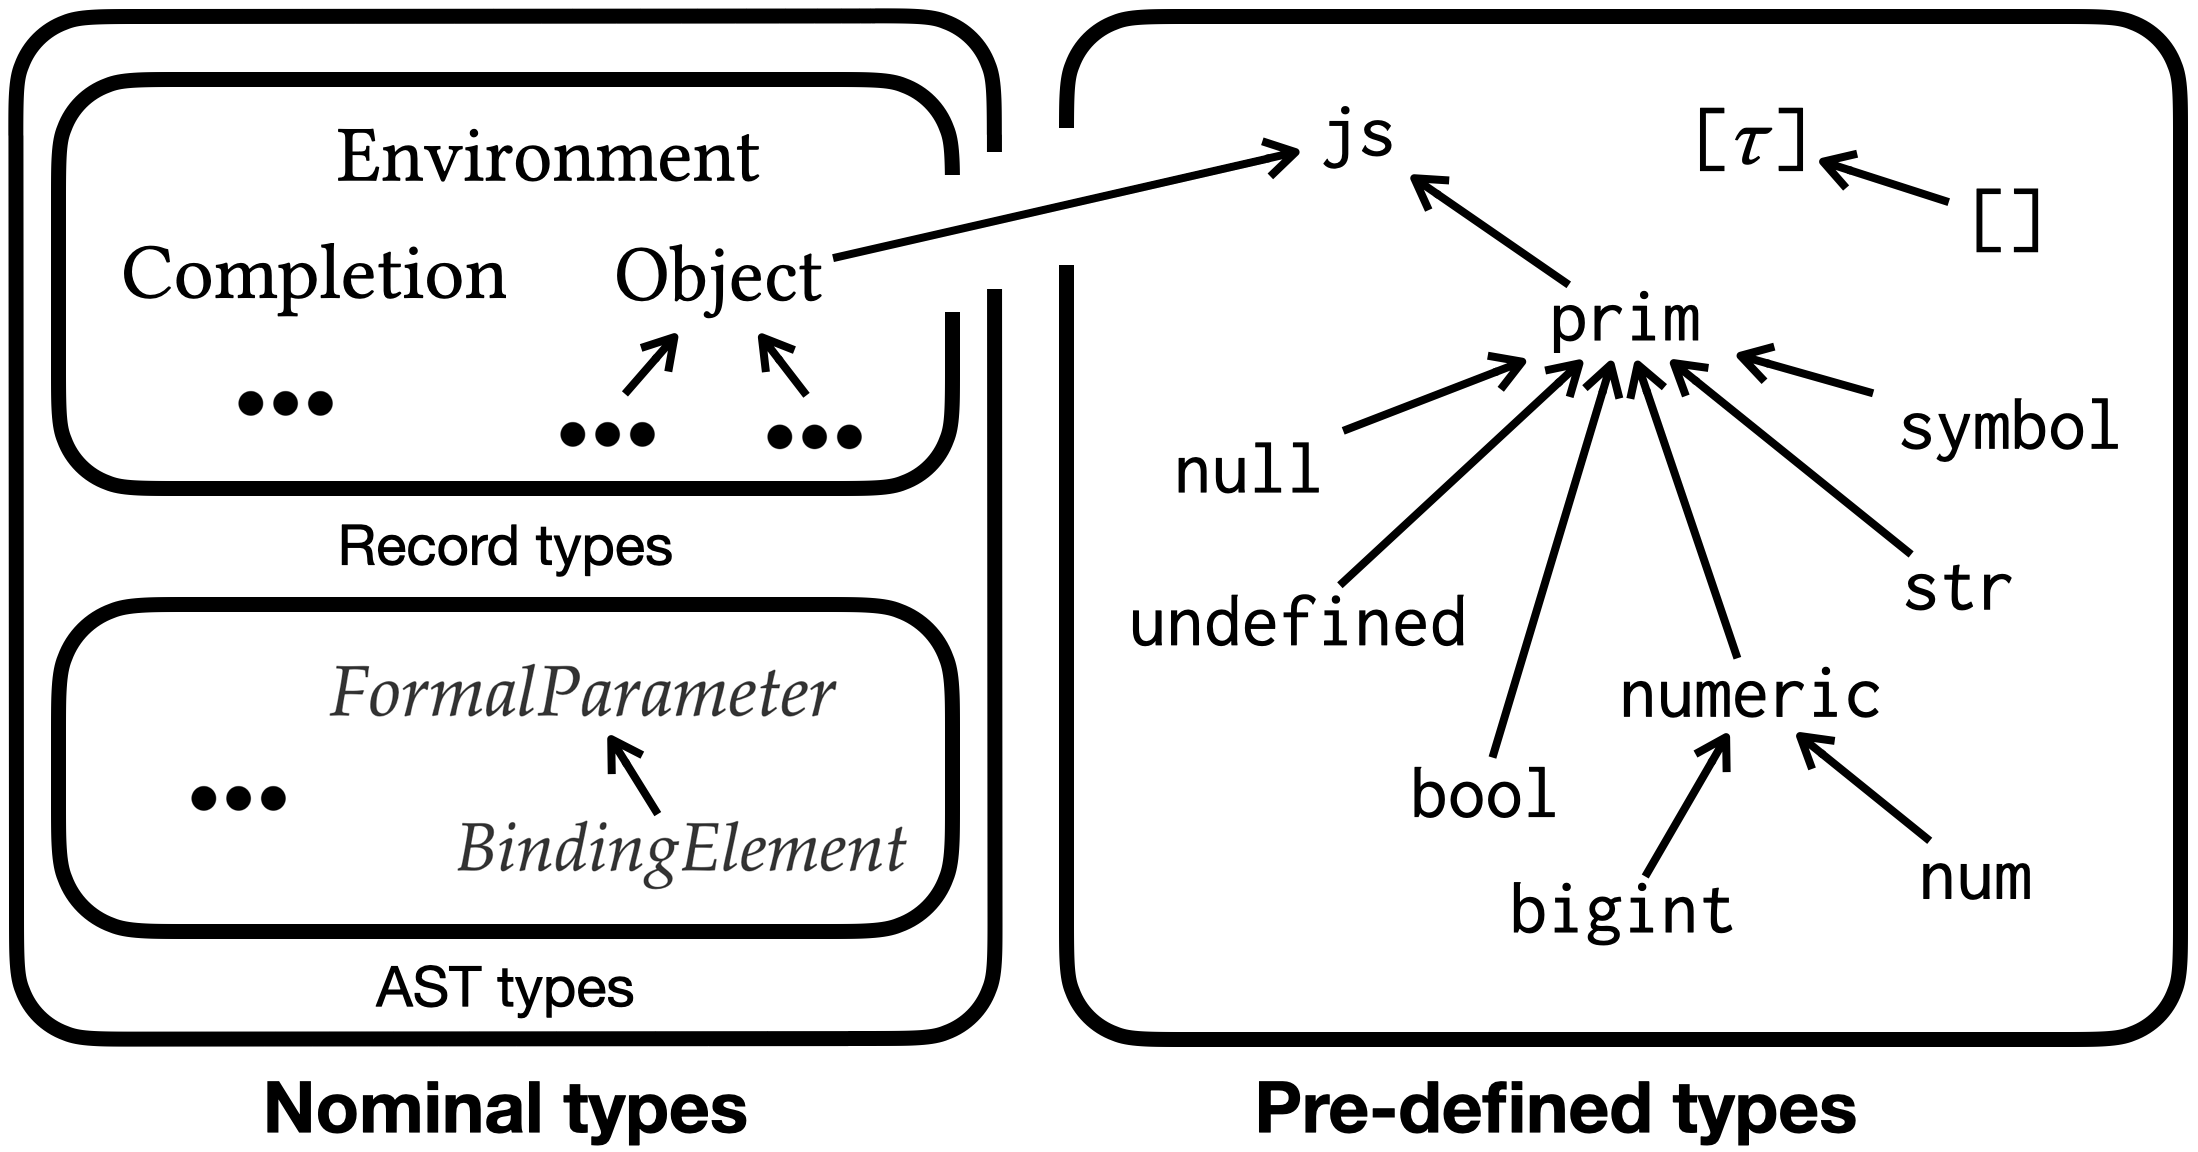
\includegraphics[width=0.4\textwidth]{img/subtype}
  \vspace*{-1.5em}
  \caption{A graphical representation of subtype relation $\subtype$.}
  \label{fig:subtype}
  \vspace*{-1.5em}
\end{figure}

A type $\ty \in \tyset$ is a norminal type $\tname$ or a pre-defined type;
$\tjs$ denotes JavaScript values, $\tprim$ primitives, $\tnumeric$ either Number
or BigInt values, and $\tnum$, $\tbigint$, $\tstr$, and $\tsymb$ denote Number,
BigInt, String, and Symbol values, respectively.  A norminal type $\tname$ is
either 1) a \textit{production type} for ASTs or 2) a \textit{record type} used
in abstract algorithms, and ECMAScript describes its fields with pre-defined or
possible values.  A production type has corresponding syntax-directed algorithms
as its fields and a record type has specific fields with possible values
described in the corresponding table and additional description in ECMAScript.
The production type is automatically extracted but we manually model fields of
record types.  For example, Figure~\label{fig:record-fields-table} is an excerpt
from ES11 that describes fields of completion
records~\footnote{https://262.ecma-international.org/11.0/\#table-8}; it
contains three fields ``Type'' with a constant such as \code{normal}, ``Value''
with JavaScript values or an constant \code{empty}, and ``Target'' with String
values or \code{empty}.  We manually model them as follows:
\small
\[
  \begin{array}{l}
    \text{Completion} = \kwcl\\
    \quad \Type: \kwcl \nconst{normal}, \nconst{break}, \nconst{continue},
    \nconst{return}, \nconst{throw} \kwcr\\
    \quad \Value: \kwcl \tjs, \nconst{empty} \kwcr\\
    \quad \Target: \kwcl \tstr, \nconst{empty} \kwcr\\
    \kwcr\\
  \end{array}
\]

The subtype relation $\subtype \subseteq \tyset \times \tyset$ between types is
depicted in Figure~\ref{fig:subtype}; the directed edge from $\ty'$ to $\ty$
denotes $\ty' \subtype \ty$ and the relation is reflexive and transitive.  The
subtype relation is dependent on the syntax and defined record types in
ECMAScript.  We extract subtypes for production types and manually model
subtypes between record types.  For example, consider the syntax-directed
abstract algorithm at the lower-right in Figure~\ref{fig:example}.  The
non-terminal \textit{BindingElement} is the unique token in a alternative of
\textit{FormalParameter} production thus we automatically extract the subtype
relation: \textit{BindingElement} $\subtype$ \textit{FormalParameter}.  Based on
this subtype relation, a type check expression $\expr: \ty$ checks whether the
evaluation result of $\expr$ has a type $\ty'$ satisfying $\ty' \subtype \ty$.

We define a denotational semantics of the modified $\ires$ for instructions
$\semi{\inst}: \dom \rightarrow \dom$, references $\semr{\refer}: \dom
\rightarrow \valset$, and expressions $\seme{\expr}: \dom \rightarrow \valset$.
For presentation brevity, we omit it in this paper and include it in a companion
report~\inred{\cite{report}}.


\subsection{Type Analysis}\label{sec:analysis}

\begin{figure*}[t]
  \centering
  \begin{subfigure}[b]{\textwidth}
    \[
      \begin{array}{r@{~}c@{~}ll}
        \asemi{\kwlet \; \x = \expr}
        (\lab, \tys)(\aelem) &=&
        (\{ (\getnext(\lab), \tys) \mapsto \aenv_\x \}, \emp) &
        \text{where} \;
        \aenv_\x = \aenv[\x \mapsto \aty] \wedge
        \aty = \aseme{\expr}(\aenv)\\

        \asemi{\x = \kwrl \expr_0 \; \expr_1 \cdots \expr_n \kwrr}
        (\lab, \tys)(\aelem) &=&
        \left(
          \begin{array}{@{}l@{}}
            \{ (\lab_\func, \tys_a) \mapsto \aenv_{\func, \tys_a} \mid \func \in
              F \wedge \tys_a \in T_a
            \},\\
            \{ (\func, \tys_a) \mapsto \{ (\getnext(\lab), \tys, \x) \} \mid
              \func \in F \wedge \tys_a \in T_a
            \}\\
          \end{array}
        \right) &
        \text{where} \;
        \left\{
          \begin{array}{@{}l@{}}
            \aty_i = \aseme{\expr_i}(\aenv) \wedge T_a = \{ \upcasts([ \ty_1,
            \cdots, \ty_n ] \mid \ty_i \in \aty_i \} \wedge\\
            F = \{ \func \in \aty_0 \mid \func = \kwdef \; \_ (\p_1, \cdots,
            \kwsl \cdots, \p_m \kwsr). \; \lab_\func \} \wedge\\
            \aenv_{\func, \tys_a} = \aenv[\p_1 \mapsto \{ \tys_a[1] \}, \cdots,
            \p_m \mapsto \{ \tys_a[m] \}]\\
          \end{array}
        \right.\\

        \asemi{\kwassert \; \expr}
        (\lab, \tys)(\aelem) &=&
        (\{ (\getnext(\lab), \tys) \mapsto \aenv_\mt \}, \emp) &
        \text{where} \; \aenv_\mt = \refine(\expr, \true)(\aenv)\\

        \asemi{\kwif \; \expr \; \lab_\mt \; \lab_\mf}
        (\lab, \tys)(\aelem) &=&
        (\{ (\lab_\mt, \tys) \mapsto \aenv_\mt, (\lab_\mf, \tys) \mapsto
        \aenv_\mf \}, \emp) &
        \text{where} \;
        \aenv_\mt = \refine(\expr, \true)(\aenv) \wedge
        \aenv_\mf = \refine(\expr, \false)(\aenv)\\

        \asemi{\kwreturn \; \expr}
        (\lab, \tys)(\aelem) &=&
        (\{ (\lab_r, \tys_r) \mapsto \aenv_r \mid (\lab_r, \tys_r, \x) \in
        \retp(\getfunc(\lab), \tys)\}, \emp) &
        \text{where} \;
        \aelem = (\rmap, \retp) \wedge
        \aenv_r = \rmap(\lab_r, \tys_r)[\x \mapsto \aty] \wedge
        \aty = \aseme{\expr}(\aenv)\\

        \asemi{\x = \expr}
        (\lab, \tys)(\aelem) &=&
        (\{ (\getnext(\lab), \tys) \mapsto \aenv_\x \}, \emp) &
        \text{where} \;
        \aenv_\x = \aenv[\x \mapsto \aty] \wedge
        \aty = \aseme{\expr}(\aenv)\\

        \asemi{\refer \kwsl \expr_0 \kwsr = \expr_1}
        (\lab, \tys)(\aelem) &=&
        (\{ (\getnext(\lab), \tys) \mapsto \aenv \}, \emp)
      \end{array}
    \]
    \caption{Instructions with $\asemi{\inst}: (\labset \times \tyset^*)
    \rightarrow \adom \rightarrow \adom$ where $\aenv = \aelem(\lab, \tys)$.}
  \end{subfigure}
  \begin{subfigure}[b]{0.48\textwidth}
    \[
      \asemr{\x}(\aenv) = \aenv(\x)
      \qquad
      \asemr{\refer \kwsl \expr \kwsr}(\aenv) = \{ \ty[\str] \mid \ty \in
      \asemr{\refer}(\aenv) \wedge \str \in \aseme{\expr}(\aenv) \}
    \]
    \caption{References with $\asemr{\refer}: \aenvset \rightarrow \atyset$.}
  \end{subfigure}
  \begin{subfigure}[b]{\textwidth}
    \[
      \begin{array}{r@{~}c@{~}lr@{~}c@{~}lr@{~}c@{~}l}
        \aseme{\tname \; \kwcl \fields \kwcr}(\aenv)
        &=& \multicolumn{7}{@{}l}{
          \left\{
            \begin{array}{ll}
              \{ \tnormal(\ty) \mid \ty \in \aseme{\fields(\code{Value})}(\aenv)
              \} & \text{if} \; \tname = \text{Completion} \wedge
              \fields(\code{Type}) = \nconst{normal}\\

              \{ \tabrupt \} & \text{if} \; \tname = \text{Completion} \wedge
              \fields(\code{Type}) \neq \nconst{normal}\\

              \{ \tname \} & \text{otherwise}\\
            \end{array}
          \right.
          \quad \aseme{\prim}(\aenv) =
          \left\{
            \begin{array}{ll}
              \{ \tnum \} & \text{if} \; \prim = \num\\
              \{ \tbigint \} & \text{if} \; \prim = \bigint\\
              \{ \tsymb \} & \text{if} \; \prim = \symb\\
              \{ \prim \} & \text{otherwise}\\
            \end{array}
          \right.
        }

        \\

        \aseme{\const}(\aenv) &=& \const &

        \aseme{\clist{}}(\aenv) &=& \clist{} &

        \aseme{\clist{\expr_0, \cdots, \expr_n}}(\aenv)
        &=& \{ \clist{\ty} \mid \ty \in \bigjoin_{0 \leq i
        \leq n} \aseme{\expr_i}(\aenv) \}

        \\

        \aseme{\expr: \ty}(\aenv)
        &=& \{ \ty' \subtype \ty \mid \ty' \in
        \aseme{\expr}(\aenv) \} &

        \aseme{\refer \kwexists}(\aenv)
        &=& \{ \ty \neq \tabsent \mid \ty \in
        \aseme{\expr}(\aenv) \} &

        \aseme{\refer}(\aenv)
        &=& \asemr{\refer}(\aenv) \setminus \{ \tabsent \}

        \\

        \aseme{\uop \; \expr}(\aenv)
        &=& \{ \abs{\uop} \ty \mid \ty \in
        \aseme{\expr}(\aenv) \} &

        \aseme{\expr_0 \bop \expr_1}(\aenv)
        &=& \multicolumn{4}{@{}l}{\{ \ty_0 \abs{\bop} \ty_1 \mid \ty_0 \in
        \aseme{\expr_0}(\aenv) \wedge \ty_1 \in \aseme{\expr_1}(\aenv) \}}

        \\
      \end{array}
    \]
    \caption{Expressions with $\aseme{\expr}: \aenvset \rightarrow \atyset$.}
  \end{subfigure}
  \caption{Abstract semantics of the modified $\ires$ for a program $\prog =
  (\getfunc, \getinst, \getnext)$.}
  \vspace*{-1.5em}
  \label{fig:abs-sem}
\end{figure*}

We design a type analysis for the modified $\ires$ based on abstract
interpretation framework~\cite{ai1977, ai1992} with analysis
sensitivity~\cite{sens-toplas}.  We first extend types $\tyset$ as follows:
\[
  \tyset \ni \ty ::=
  \cdots \mid
  \func \mid
  \const \mid
  \tnormal(\ty) \mid
  \tabrupt \mid
  \bool \mid
  \str \mid
  \tabsent
\]
There are three different reasons why we extend types.  First, the original
types $\tyset$ do not cover all types of values thus we add functions and
constants.  Second, we add more specific types to increase the precision of type
analysis.  A completion record is a \textit{normal completion} when its Type
field is a constant $\nconst{normal}$ or an \textit{abrupt completion}
otherwise.  We add $\tnormal(\ty)$ and $\tabrupt$ for normal and abrupt
completions.  Moreover, we also add Boolean values $\bool$, and String values
$\str$ to precisely handle the control flows of branches and field accesses,
respectively.  Third, we add the absent type $\tabsent$ to represent the
existence of variables.  Using such extended types, we define abstract states
with flow-sensitivity and type-sensitivity for parameters:
\[
  \begin{array}{lr@{~}c@{~}c@{~}r@{~}l}
    \text{Abstract States}
    &\aelem&\in&\adom&=& \rmapset \times \retpset\\

    \text{Result Maps}
    &\rmap&\in&\rmapset&=& \labset \times \tyset^* \rightarrow \aenvset\\

    \text{Return Points}
    &\retp&\in&\retpset&=& \funcset \times \tyset^*
    \rightarrow \partsof{\labset \times \tyset^* \times \varset} \\

    \text{Abstract Environments}
    &\aenv&\in&\aenvset&=&\varset \rightarrow \atyset\\

    \text{Abstract Types}
    &\aty&\in&\atyset&=&\partsof{\tyset}\\
  \end{array}
\]
An abstract state $\aelem \in \adom$ is pair of a return map and a return point
mapping.  A result map $\rmap \in \rmapset$ represents an abstract environment
for each flow-sensitive and type-sensitive view, and a return point mapping
$\retp \in \retpset$ represents possible return points of each function with
a type-sensitive context.  An abstract environment $\aenv \in \aenvset$
represents possible types of each variable, and $\aenv(\x) = \{ \tabsent \}$
when $\x$ is not defined in $\aenv$.  An abstract type $\aty \in \atyset$ is a
set of types.  While we define the join operator $\join$, the meet operator
$\meet$, and the partial order $\order$ for most of abstract domains in a
point-wise manner, we define the operators for types with a normalization
function $\norm$ because of their subtype relations:
\[
  \begin{array}{l}
    \aty_0 \join \aty_1 = \norm(\aty_0 \cup \aty_1)\\
    \aty_0 \meet \aty_1 = \norm(
      \{\ty_0 \in \aty_0 \mid \{ \ty_0 \} \order \aty_1 \} \cup
      \{\ty_1 \in \aty_1 \mid \{ \ty_1 \} \order \aty_0 \}
    )\\
    \aty_0 \order \aty_1 \Leftrightarrow \forall \ty_0 \in \aty_0. \; \exists
    \ty_1 \in \norm(\aty_1). \; \text{s.t.} \; \ty_0 \subtype \ty_1\\
  \end{array}
\]
where $\norm(\aty) = \{ \ty \mid \ty \in \aty_e \wedge \not\exists \ty' \in
\aty_e. \; \text{s.t.} \; \ty \neq \ty' \wedge \ty \subtype \ty' \}$.

Based on abstract states, we define the abstract semantics of instructions,
references, and expressions in the modified $\ires$ described in
Figure~\ref{fig:abs-sem}.  To prevent the explosion of the number of type-sensitive
views, we upcast the type of each argument before function calls with the
following function:
\[
  \upcast(\ty) = \left\{
    \begin{array}{ll}
      \tnormal(\upcast(\ty')) & \text{if} \; \ty = \tnormal(\ty')\\
      \clist{\upcast(\ty')} & \text{if} \; \ty = \clist{\ty'}\\
      \tstr & \text{if} \; \ty = \str\\
      \tbool & \text{if} \; \ty = \bool\\
      \ty & \text{otherwise}\\
    \end{array}
  \right.
\]
and $\upcasts$ denotes a point-wise extension of $\upcast$ for type sequences.
For branches and assertions, we apply the $\refine$ function that prunes out
infeasible parts in abstract environments based on their conditions to increase
analysis precision.  We explain its detail in Section~\ref{sec:refine}.  Then,
we define the abstract semantics $\asem{\prog}$ of a program $\prog = (\getfunc,
\getinst, \getnext)$ as the least fixpoint of abstract transfer $\atransfer:
\adom \rightarrow \adom$:
\[
  \begin{array}{r@{~}c@{~}l}
    \asem{\prog} &=& \lim_{n \rightarrow \infty}(\atransfer)^n(\iaelem)\\
    \atransfer(\aelem) &=& \aelem \join \left(
      \underset{(\lab, \tys) \in \domain{\rmap}}{\bigjoin}
      \asemi{\getinst(\lab)}(\lab, \tys)(\aelem)
    \right)\\
  \end{array}
\]
where $\aelem = (\rmap, \_)$ and $\iaelem$ denotes the initial abstract state.
As described in the Section~\ref{sec:overview}, $\iaelem$ contains all
syntax-directed algorithms having no additional parameters and built-in
algorithms with appropriate abstract environments.  For syntax-directed
algorithms, we construct its abstract environment containing the variable
$\this$ with a production type and other variables for non-terminals.  For
example, the upper-left syntax-directed algorithm in Figure~\ref{fig:example} is
initialized with the following abstract environment:
\[
  \left\{
    \begin{array}{r@{~}c@{~}l}
      \this &\mapsto& \{ \text{AssignmentExpression} \},\\
      \mcode{LeftHandSideExpression} &\mapsto& \{ \text{LeftHandSideExpression} \},\\
      \mcode{AssignmentExpression} &\mapsto& \{ \text{AssignmentExpression} \}
    \end{array}
  \right.
\]
For built-in algorithms, we assign pre-defined variables $\this$, $\args$, and
$\NewTarget$ with corresponding types and parameters with $\tjs$ types.  For
example, the following abstract environment is for the built-in
algorithm $\jscode{Math.round}$ at the upper-right in Figure~\ref{fig:example}:
\[
  \left\{
    \begin{array}{r@{~}c@{~}l}
      \this &\mapsto& \{ \tjs \},
      \args \mapsto \{ \clist{\tjs} \},
      \x \mapsto \tjs\\
      \NewTarget &\mapsto& \{ \text{Object}, \undefval \},\\
    \end{array}
  \right.
\]


\subsection{Condition-based Refinement}\label{sec:refine}

We present a \textit{condition-based refinement} of type analysis for the
modified $\ires$ to increase analysis precision.  It prunes out infeasible parts
in abstract environments based on conditions of branches of assertions, and we
formally define the $\refine$ function as a composition of two functions
$\refineFlow$ and $\refineVar$:
\[
  \refine(\expr, \bool) =
  \refineVar(\expr, \bool) \circ \refineFlow(\expr, \bool)
\]
The $\refineFlow$ prevents infeasible \textit{control flows} by producing an
empty abstract environment as follows:
\[
  \refineFlow(\expr, \bool)(\aenv) = \left\{
    \begin{array}{ll}
      \aenv & \text{if} \; \{ \bool \} \order \aseme{\expr}(\aenv)\\
      \emp & \text{otherwise}\\
    \end{array}
  \right.
\]
Beyond control flows, $\refineVar$ refines the shape of a given abstract
environment based on the conditions for variables:
\[
  \begin{array}{r@{~}c@{~}l}
    \refineVar(\code{!} \expr, \bool)(\aenv) &=&
    \refineVar(\expr, \neg \bool)(\aenv)\\

    \refineVar(\expr_0 \bop \expr_1, \bool)(\aenv) &=&
    \left\{
      \begin{array}{ll}
        \aenv_0 \join \aenv_1 & \text{if} \; \bool \wedge \bop = \code{||}\\
        \aenv_0 \meet \aenv_1 & \text{if} \; \neg\bool \wedge \bop = \code{||}\\
        \aenv_0 \meet \aenv_1 & \text{if} \; \bool \wedge \bop = \code{\&\&}\\
        \aenv_0 \join \aenv_1 & \text{if} \; \neg\bool \wedge \bop = \code{\&\&}\\
        \aenv & \text{otherwise}\\
      \end{array}
    \right.\\
    \multicolumn{3}{r}{
      \text{where} \;
      \aenv_0 = \refineVar(\expr_0, \bool)(\aenv) \wedge
      \aenv_1 = \refineVar(\expr_1, \bool)(\aenv)
    }\\

    \refineVar(\x.\Type \code{=} \nconst{normal}, \true)(\aenv) &=&
    \aenv[ \x \mapsto \aseme{\x}(\aenv) \cap \tnormal(\tyset) ]\\
    \refineVar(\x.\Type \code{=} \nconst{normal}, \false)(\aenv) &=&
    \aenv[ \x \mapsto \aseme{\x}(\aenv) \cap \{ \tabrupt \} ]\\

    \refineVar(\x \code{=} \expr, \true)(\aenv) &=&
    \aenv[ \x \mapsto \aseme{\x}(\aenv) \meet \aseme{\expr}(\aenv) ]\\
    \refineVar(\x \code{=} \expr, \false)(\aenv) &=&
    \aenv[ \x \mapsto \aseme{\x}(\aenv) \setminus
    \lfloor\aseme{\expr}(\aenv)\rfloor ]\\

    \refineVar(\x : \ty, \true)(\aenv) &=&
    \aenv[ \x \mapsto \aseme{\x}(\aenv) \meet \{ \ty \} ]\\
    \refineVar(\x : \ty, \false)(\aenv) &=&
    \aenv[ \x \mapsto \aseme{\x}(\aenv) \setminus \{ \ty' \mid \ty' \subtype \ty
    \}]\\
  \end{array}
\]
and it returns $\aenvset$ for other cases.  The notation $\getSingle{\aty}$ denotes
to checks whether it is a singleton; $\getSingle{\aty} = \aty$ if $\aty = \{ \ty
\}$ and $\ty$ is a singleton type such as a constant $\const$, an empty list
$\clist{}$, an absent value $\tabsent$, a primitive value, etc., and
$\getSingle{\aty} = \emp$ otherwise.

\section{Bug Detector}\label{sec:checker}

\begin{table}
  \centering
  \caption{Type-related specification bugs fixed by pull requests for the recent
  three years from 2018 to 2021.}
  \label{table:pr-bugs}
  \vspace*{-1.5em}
  \[
    \small
    \begin{array}{c|l|r|r}
      \multicolumn{1}{c|}{\textbf{Category}} &
      \multicolumn{1}{c|}{\textbf{Bug Kind}} &
      \multicolumn{1}{c|}{\textbf{\# PR}} &
      \multicolumn{1}{c}{\textbf{\# Bugs}}\\
      \hline

      \multirow{2}{*}{\text{Reference}}
      & \text{Unknown Variables} & \inred{XXX} & \inred{XXX}\\\cline{2-4}
      & \text{Already Defined Variables} & \inred{XXX} & \inred{XXX}\\\hline

      \multirow{1}{*}{\text{Parameter}}
      & \text{Arity Mismatches} & \inred{XXX} & \inred{XXX}\\\hline

      \multirow{1}{*}{\text{Assertion}}
      & \text{Assertion Failures} & \inred{XXX} & \inred{XXX}\\\hline

      \multirow{2}{*}{\text{Type}}
      & \text{Non-Numeric Operands} & \inred{XXX} & \inred{XXX}\\\cline{2-4}
      & \text{Unchecked Abrupt Completions} & \inred{XXX} & \inred{XXX}\\\hline

      \multicolumn{2}{c|}{\textbf{Total}} & \inred{XXX} & \inred{XXX}\\

    \end{array}
  \]
  \vspace*{-1.5em}
\end{table}

% TODO: more detail of investigation

We develop a \textit{bug detector} to statically detect type-related
specification bugs in ECMAScript using an augmented abstract transfer
$\detector$ with additional checkers.  The abstract semantics $\asem{\prog}$ of
a program $\prog = (\getfunc, \getinst, \getnext)$ is the least fixpoint of the
original abstract transfer $\atransfer$.  Thus, $\detector(\asem{\prog})$ also
produces $\asem{\prog}$ and detects type-related specification bugs.  Before
implementing checkers, we manually investigate pull requests for the recent
\inred{three years from 2018 to 2021}.  As described in
Table~\ref{table:pr-bugs}, \inred{XXX} pull requests existed having bugfixes of
\inred{XXX} type-related specification bugs classified in six different kinds
and four categories.  To detect such specification bugs, we implement four
checkers for each category of bugs: \textit{reference checker}, \textit{arity
checker}, \textit{assertion checker}, and \textit{operand type checker}.  Now,
we explain how each checker detects corresponding bugs in the augmented abstract
transfer $\detector$.


\subsection{Reference Checker}

In ECMAScript abstract algorithms, variables are dynamically introduced in any
contexts.  A \textit{reference bug} occurs when trying to access a not yet
defined variable or to redefine an already defined variable.  According to our
manual investigation of pull requests, the reference bug is the most prevalent
type-related specification bugs; \inred{XXX} pull requests fixed \inred{XXX}
unknown variable bugs and \inred{XXX} pull requests fixed \inred{XXX} already
defined variable bugs.  We implement the reference checker by adding additional
checks to abstract semantics of variable lookups $\aseme{\x}$ and variable
declarations $\asemi{\kwlet \; \x = \expr}$ to detect unknown variables and
already defined variables, respectively:
\[
  \small
  \begin{array}{r@{~}c@{~}l}
    \aseme{\x}(\aenv) &=& \left\{
      \begin{array}{ll}
        \text{unknown variable} \; $\x$
        & \text{if} \; \asemr{\x}(\aenv) = \{ \tabsent \}\\
        \cdots
        & \text{otherwise}\\
      \end{array}
    \right.\\

    \asemi{\kwlet \; \x = \expr}(\lab, \tys)(\aelem) &=& \left\{
      \begin{array}{ll}
        \text{already defined variable} \; $\x$
        & \text{if} \; \aty = \{ \true \}\\
        \cdots
        & \text{otherwise}\\
      \end{array}
    \right.\\ &&
    \text{where} \; \aty = \aseme{\x \kwexists}(\aelem(\lab, \tys))\\
  \end{array}
\]
If the abstract semantics of a variable lookup for $\x$ is a singleton $\{
\tabsent \}$, it means the variable $\x$ is always an unknown variable.  In this
case, the reference checker reports an unknown variable bug for $\x$.  For
example, consider the syntax-directed algorithm at the upper-left in
Figure~\ref{fig:example}.  Since the \textbf{GetReferencedName} algorithm is
removed, the variable \code{GetReferencedName} does not exist in abstract
environments and its lookup returns $\{ \tabsent \}$ thus the reference checker
reports the unknown variable bug for \code{GetReferencedName}.  For already
defined variables, the reference checker utilizes the abstract semantics of
existence check $\aseme{\x \kwexists}$ to check whether the variable $\x$ in
each variable declaration is already defined.


\subsection{Arity Checker}

Arity $\size{\func}$ of a function $\func = \kwdef \; \f (\p_1, \cdots, \p_n,
\kwsl \cdots, p_m \kwsr). \; \lab$ is defined as an interval $[n, m]$ where $n$
and $m-n$ denote numbers of normal and optional parameters, respectively.  In
function invocations, an \textit{arity mismatch} occurs when the number of
arguments is not matched with the arity of a function, and \inred{XXX} pull
requests fixed \inred{XXX} arity mismatches.  The arity checker detects such
arity mismatches by using additional checks in the abstract semantics of
function call instructions $\asemi{\x = \kwrl \expr_0 \; \expr_1 \cdots \expr_k
\kwrr}$:
\[
  \small
  \begin{array}{l}
    \asemi{\x = \kwrl \expr_0 \; \expr_1 \cdots \expr_k \kwrr}(\lab,
    \tys)(\aelem) =\\
    \qquad \left\{
      \begin{array}{ll}
        \text{missing parameters} \; \p_{k+1}, \cdots, \p_{n_\func} &
        \text{if} \; \exists \func \in \aty_0. \; \text{s.t.} \; k < n_\func\\

        \text{remaining arguments} \; \expr_{m_\func+1}, \cdots, \expr_k &
        \text{if} \; \exists \func \in \aty_0. \; \text{s.t.} \; k > m_\func\\

        \cdots &
        \text{otherwise}\\
      \end{array}
    \right.\\
  \end{array}
\]
where $\func = \kwdef \; \f (\p_1, \cdots, \p_{n_\func}, \kwsl \cdots,
p_{m_\func} \kwsr). \; \lab \wedge \aty_0 = \aseme{\expr_0}(\aelem(\lab,
\tys))$.  For each function $\func$ in the abstract semantics of the function
expression $\expr_0$, the arity checker compares the number of arguments with
the arity $\size{\func}$ to detect arity mismatches.  For example, consider the
lower-left syntax directed algorithm in Figure~\ref{fig:example}.  The algorithm
invocation in line 2 is compiled to a function call instruction:
\[
  \small
  \x = \kwrl \code{formal}.\code{IteratorBindingInitialization} \; \code{formal}
  \kwrr
\]
with a temporal variable $\x$.  While it passes only a single argument
$\code{formal}$, the arity of the function
$\code{formal}.\code{IteratorBindingInitialization}$ is $[3, 3]$ thus the arity
checker reports missing parameter bugs for two additional parameters
$\code{iteratorRecord}$ and $\code{environment}$.


\subsection{Assertion Checker}
An \textit{assertion failure} is a specification bug that occurs when the
condition of an assertion instruction is not true.  There were \inred{XXX} pull
requests that fixed \inred{XXX} assertion failures.  The assertion checker
detects such bugs using additional checks in the abstract semantics of assertion
instructions $\asemi{\kwassert \; \expr}$:
\[
  \small
  \asemi{\kwassert \; \expr}(\lab, \tys)(\aelem) = \left\{
    \begin{array}{ll}
      \text{assertion failure} \; \expr &
      \text{if} \; \{ \true \} \norder \aty\\

      \cdots &
      \text{otherwise}\\
    \end{array}
  \right.\\
\]
where $\aty = \aseme{\expr}(\aelem(\lab, \tys))$.  It checks whether $\{ \true
\}$ does not have partial order with the abstract semantics of the condition
expression $\expr$.  For example, consider the lower-right syntax directed
algorithm in Figure~\ref{fig:example}.  The parameter $\code{environment}$ of
this algorithm has an environment record or $\undefval$.  Since type sensitivity
divides the abstract types of arguments to upcasted single types, there are two
different abstract environments whose variable $\code{environment}$ points to
$\{ \text{Environment} \}$ or $\{ \undefval \}$.  When $\code{environment}$ is
$\{ \text{Environment} \}$, the abstract semantics of assertion condition
$\code{environment = originalEnv}$ is $\{ \tbool \}$.  Even though we know that
the type of $\code{originalEnv}$ is also $\{ \text{Environment} \}$,
\text{Environment} is not a singleton type thus we cannot convince that they are
the exactly same environment.  Thus, we cannot say that the assertion must be
failed in this case.  However, if $\code{environment}$ is $\{ \undefval \}$, the
abstract semantics of the condition $\code{environment = originalEnv}$ is $\{
\false \}$ because an environment is never equal to $\undefval$.  Thus, the
assertion checker reports an assertion failure for the condition
$\code{environment = originalEnv}$.


\subsection{Operand Type Checker}

\begin{figure*}
  \centering
  \begin{subfigure}[b]{0.24\textwidth}
    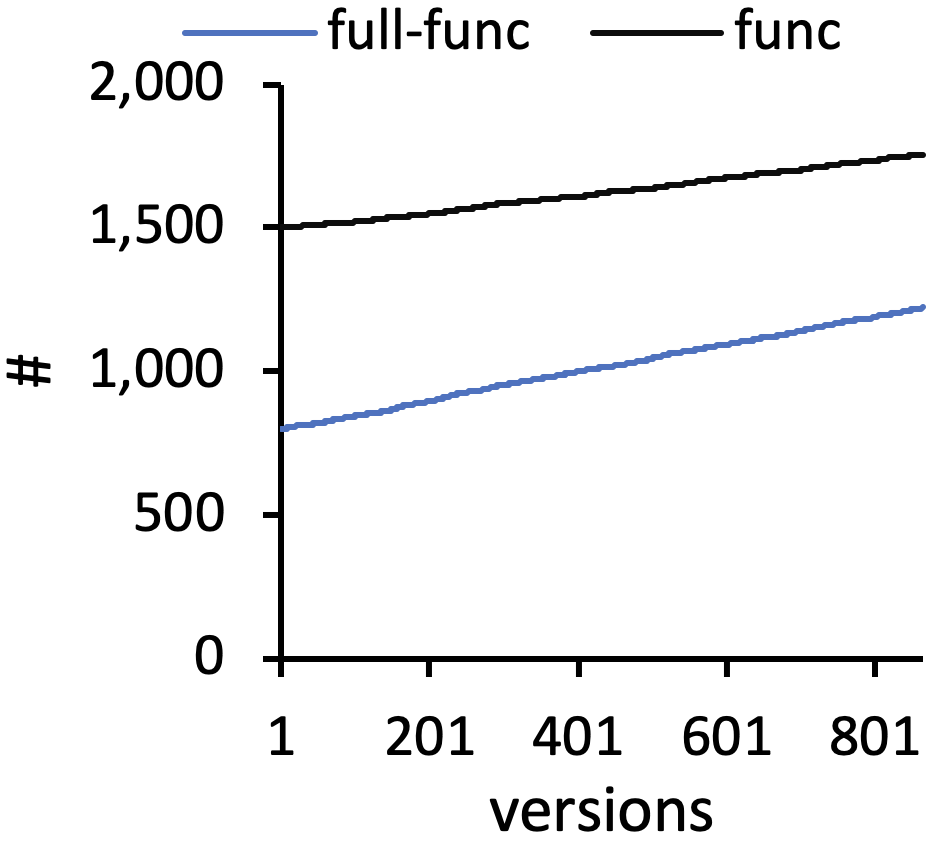
\includegraphics[width=\textwidth]{img/func}
    \caption{The number of functions.}
  \end{subfigure}
  \begin{subfigure}[b]{0.24\textwidth}
    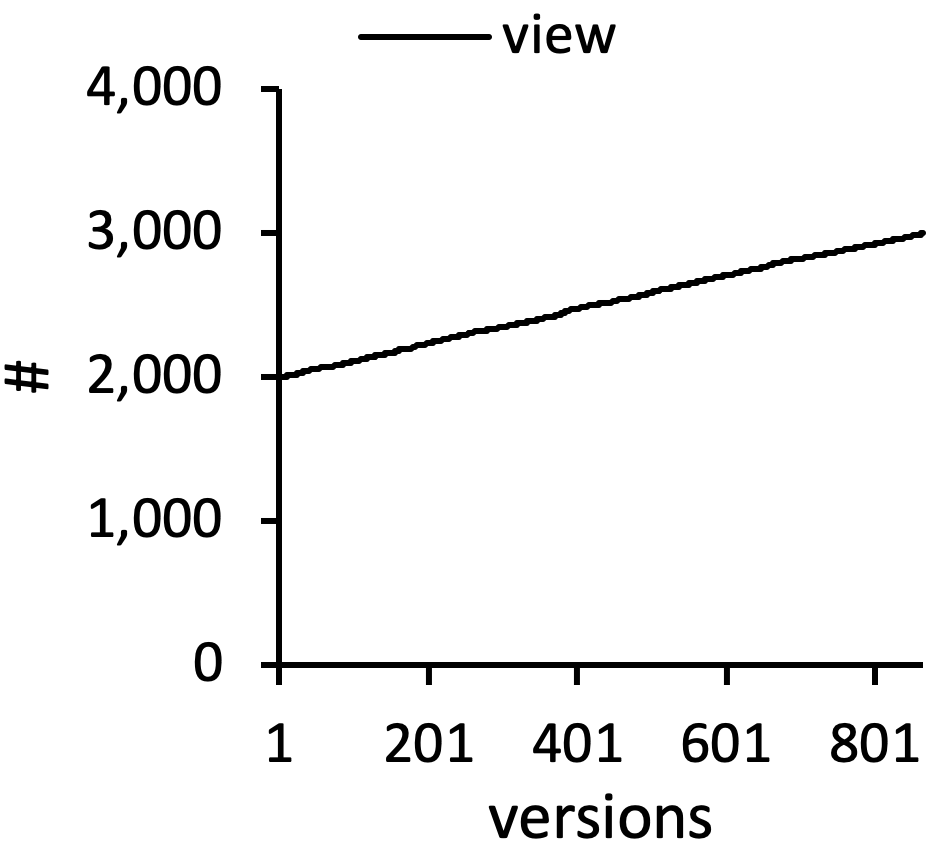
\includegraphics[width=\textwidth]{img/view}
    \caption{The number of views.}
  \end{subfigure}
  \begin{subfigure}[b]{0.24\textwidth}
    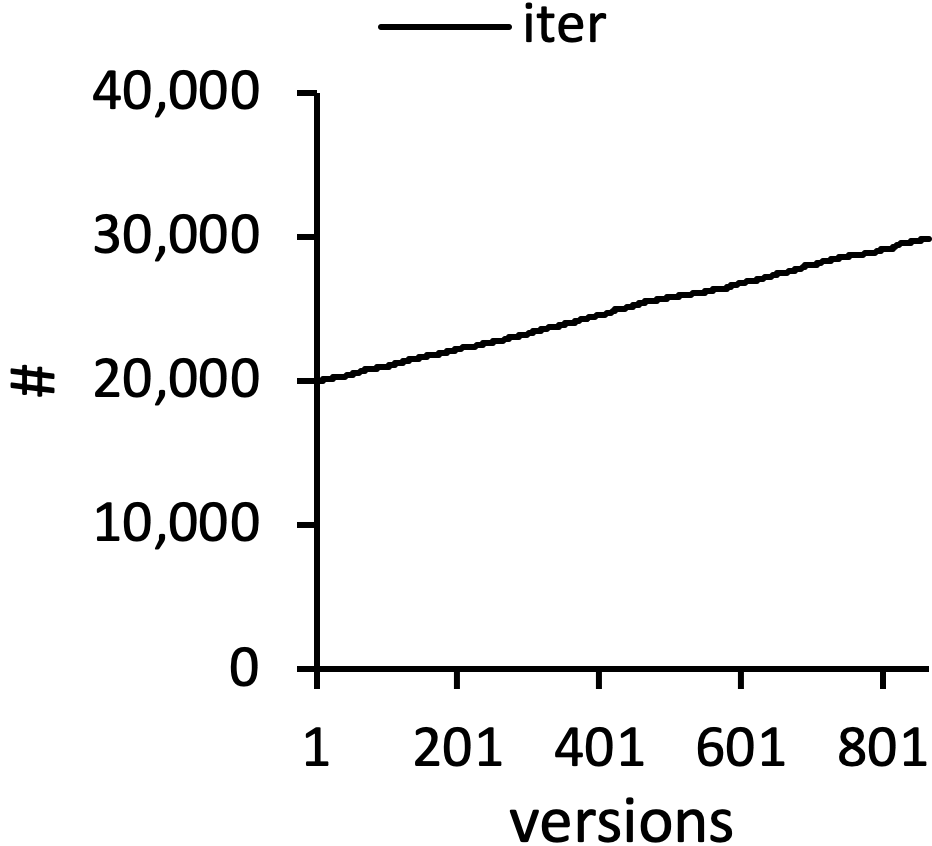
\includegraphics[width=\textwidth]{img/iter}
    \caption{The number of worklist iterations.}
  \end{subfigure}
  \begin{subfigure}[b]{0.24\textwidth}
    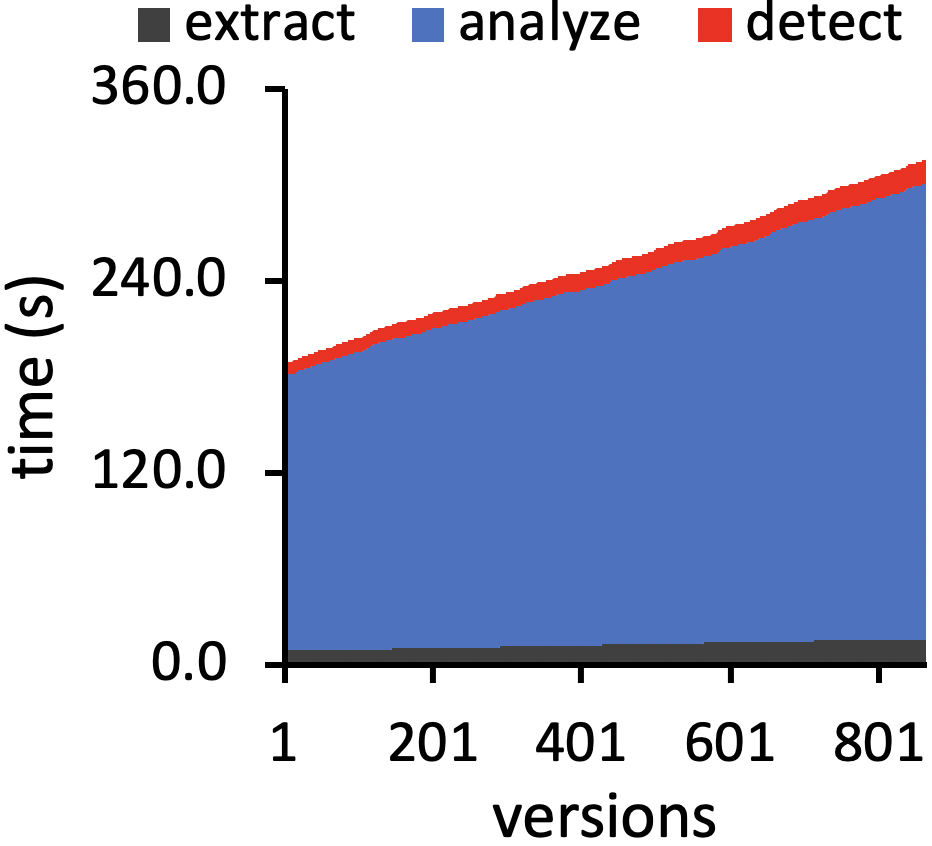
\includegraphics[width=\textwidth]{img/time}
    \caption{The analysis time.}
  \end{subfigure}
  \caption{The statistics of type analysis using $\tool$ for 864 versions of
  ECMAScript.}
  \vspace*{-1.5em}
  \label{fig:stat}
\end{figure*}

Several operators are typed and a \textit{wrong typed operand bug} occurs when
the type of an operand is not conform to the expected type.  For example, the
comparison operator $\code{<}$ is a numeric operator in the modified $\ires$.  If
an expression tries to compare between non-numeric values such as $\true <
\code{"abc"}$, then it is a non-numeric operand bug.  Besides, ECMAScript has a
special implicit conversion for normal completions when their actual values
stored in the $\code{Value}$ field are required including conditions, values of
field updates, operands of operators, etc.  For example, if the variable $\x$
has a normal completion with 42 as its actual value, $\x + 1$ should 43 because
the normal completion implicitly converted into its actual value 42.  To
explicitly represent this conversion, let's define a unary operator $\escaped$:
\[
  \small
  \escaped \val = \left\{
    \begin{array}{ll}
      \val.\code{Value} &
      \text{if} \; \val \; \text{is a normal completion}\\

      \text{unchecked abrupt completion} \; \val &
      \text{if} \; \val \; \text{is an abrupt completion}\\

      \val &
      \text{otherwise}\\
    \end{array}
  \right.
\]
and assume that the operator $\escaped$ is used when the actual value is
required.  Then, an unchecked abrupt completion bug occurs when the actual value
is required but it is an abrupt completion.  According to our manual
investigation, \inred{XXX} pull requests are related to \inred{XXX} non-numeric
operand bugs and \inred{XXX} pull requests are related to \inred{XXX} unchecked
abrupt completion bugs.

The operand checker detects such wrong typed operand bugs by using additional
checks in the abstract semantics of binary operations $\aseme{\expr \bop \expr}$
or unary operations $\aseme{\uop \; \expr}$:
\[
  \small
  \begin{array}{r@{~}c@{~}l}
    \aseme{\expr_0 \bop \expr_1}(\aenv) &=& \left\{
      \begin{array}{ll}
        \text{wrong typed operand} \; \expr_0
        & \text{if} \; \asemr{\expr_0}(\aenv) \norder \aty_0\\
        \text{wrong typed operand} \; \expr_1
        & \text{if} \; \asemr{\expr_1}(\aenv) \norder \aty_1\\
        \cdots
        & \text{otherwise}\\
      \end{array}
    \right.\\

    \aseme{\uop \; \expr}(\aenv) &=& \left\{
      \begin{array}{ll}
        \text{wrong typed operand} \; $\expr$
        & \text{if} \; \asemr{\expr}(\aenv) \norder \aty\\
        \cdots
        & \text{otherwise}\\
      \end{array}
    \right.\\
  \end{array}
\]
where $\aty_0$, $\aty_1$, and $\aty$ are expected abstract types of $\expr_0$,
$\expr_1$, and $\expr$, respectively.  The additional check reports when the
given operand does not conform to the expected types.  For example, consider the
upper-right built-in algorithm $\code{Math.round}$ in Figure~\ref{fig:example}.
The parameter $\x$ has $\{ \tjs \}$ and $\n$ has $\{ \tnum \}$ because the
\textbf{ToNumber} algorithm always return number values or abrupt completions
but later cases are removed by the \textbf{ReturnIfAbrupt} prefix ?.  While the
built-in algorithm correctly uses $\n$ in line 2, it misuses $\x$ in line 3 and
4 and $\{ \tjs \}$ does not have a partial order with the expected abstract type
$\{ \tnum, \tbigint \}$.  Thus, the operand type checker reports non-numeric
operand bugs.

\section{Evaluation}\label{sec:eval}

We developed \( \tool \) as an open source tool\footnote{The URL of the tool is
anonymized due to a double-blind review process.}, and evaluated the tool
based on the following three research questions:
\begin{itemize}[leftmargin=0.5cm]
\item RQ1. \textbf{Coverage:} How much parts \( \tool \) automatically extract
the syntax and semantics from ES7 to ES10?
\item RQ2. \textbf{Check with Tests:} The syntax and semantics of the latest
version on ECMAScript (ES10) is compatible with official tests?
\item RQ3. \textbf{Forward Compatibility:} Is \( \tool \) applicable to language
features ready for inclusion in the next ECMAScript (ES11)?
\end{itemize}


\subsection{Coverage}

\begin{table}[t]
  \caption{Number of productions in specifications,
from \textit{all} of which \( \tool \) automatically generated parsers}
  \label{fig:syntax-all-version}
\vspace*{-1em}
\small
  \[
    \begin{array}{c?r|r|r|r?r}
      \textbf{Version}
      & \multicolumn{1}{c|}{\textbf{ES7}}
      & \multicolumn{1}{c|}{\textbf{ES8}}
      & \multicolumn{1}{c|}{\textbf{ES9}}
      & \multicolumn{1}{c?}{\textbf{ES10}}
      & \multicolumn{1}{c}{\textbf{avg.}}\\\toprule
      \text{\# Lexical prod.}
      & \inred{\text{78}}
      & \inred{\text{78}}
      & \inred{\text{78}}
      & \inred{\text{81}}
      & \inred{\text{78.75}}\\\hline
      \text{\# Syntactic prod.}
      & \inred{\text{157}}
      & \inred{\text{167}}
      & \inred{\text{167}}
      & \inred{\text{174}}
      & \inred{\text{166.25}}\\
    \end{array}
  \]
  \[
    \begin{array}{c?r|r|r?r}
      \textbf{Old version}
      & \multicolumn{1}{c|}{\textbf{ES7}}
      & \multicolumn{1}{c|}{\textbf{ES8}}
      & \multicolumn{1}{c?}{\textbf{ES9}}
      & \multirow{2}{*}{\textbf{avg.}}\\\cline{1-4}
      \textbf{New version}
      & \multicolumn{1}{c|}{\textbf{ES8}}
      & \multicolumn{1}{c|}{\textbf{ES9}}
      & \multicolumn{1}{c?}{\textbf{ES10}}
      & \\\toprule
      \Delta \; \text{\# Lexical prod.}
      & \inred{\text{3}}
      & \inred{\text{5}}
      & \inred{\text{6}}
      & \inred{\text{4.67}}\\\hline
      \Delta \; \text{\# Syntactic prod.}
      & \inred{\text{140}}
      & \inred{\text{15}}
      & \inred{\text{8}}
      & \inred{\text{54.33}}\\
    \end{array}
  \]
\end{table}

\( \tool \) targets ECMAScript specifications released after ES7 in 2016 because
our tool utilizes common patterns in the converged writing style since ES7 as
already explained in Section~\ref{sec:overview}.  Thus, we evaluate the coverage
of \( \tool \) by applying it to the most recent four versions of ECMAScript,
ES7 to ES10.  We measured for how many grammar productions and steps in abstract
algorithms \( \tool \) automatically generates parsers and AST-IR translators,
respectively, in two respects: 1) in each version and 2) in each difference
between adjacent versions.

For syntax, \( \tool \) automatically generated parsers for \textit{all} the
lexical and syntactic productions.  As Table~\ref{fig:syntax-all-version} shows,
the average numbers of lexical and syntactic productions are \inred{78.75} and
\inred{166.25}, respectively.  Also, the average numbers of annually updated
lexical and syntactic productions between adjacent versions are \inred{4.67} and
\inred{54.33}, respectively.

\begin{figure}[t]
  \centering
  \begin{subfigure}{0.48\textwidth}
    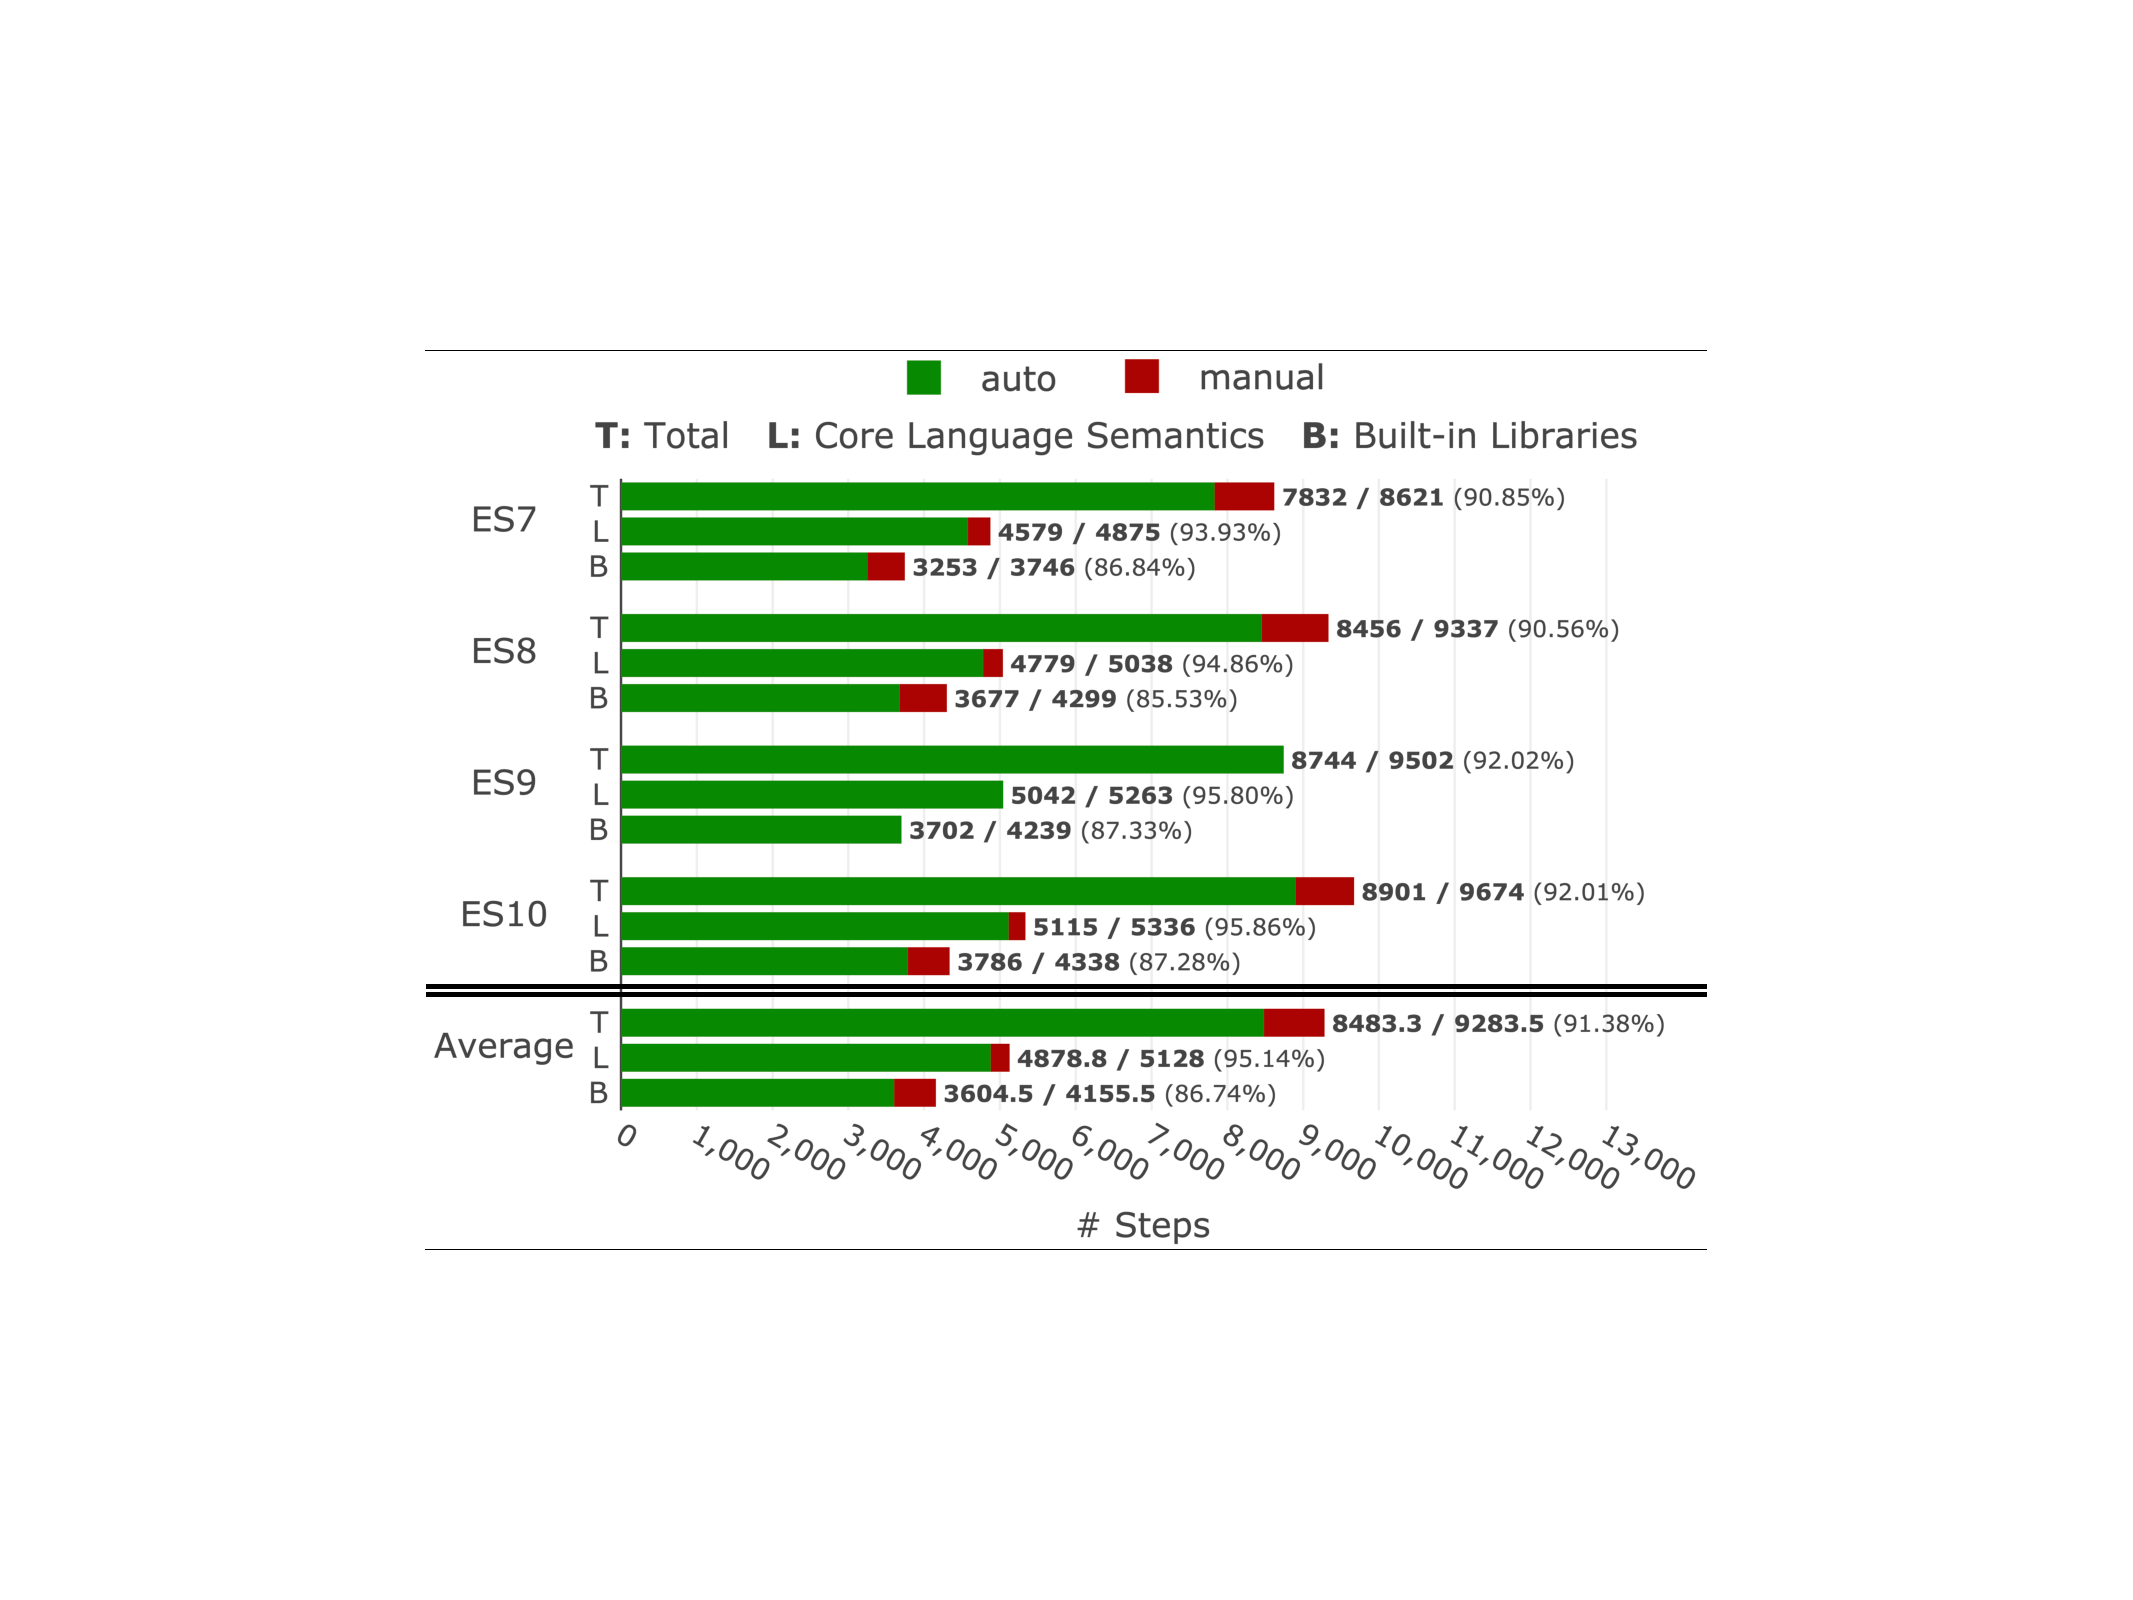
\includegraphics[width=\textwidth]{img/sem-all.pdf}
    \caption{Results for existing versions}
    \label{fig:semantics-all-version}
  \end{subfigure}
  \hfill
  \begin{subfigure}{0.48\textwidth}
    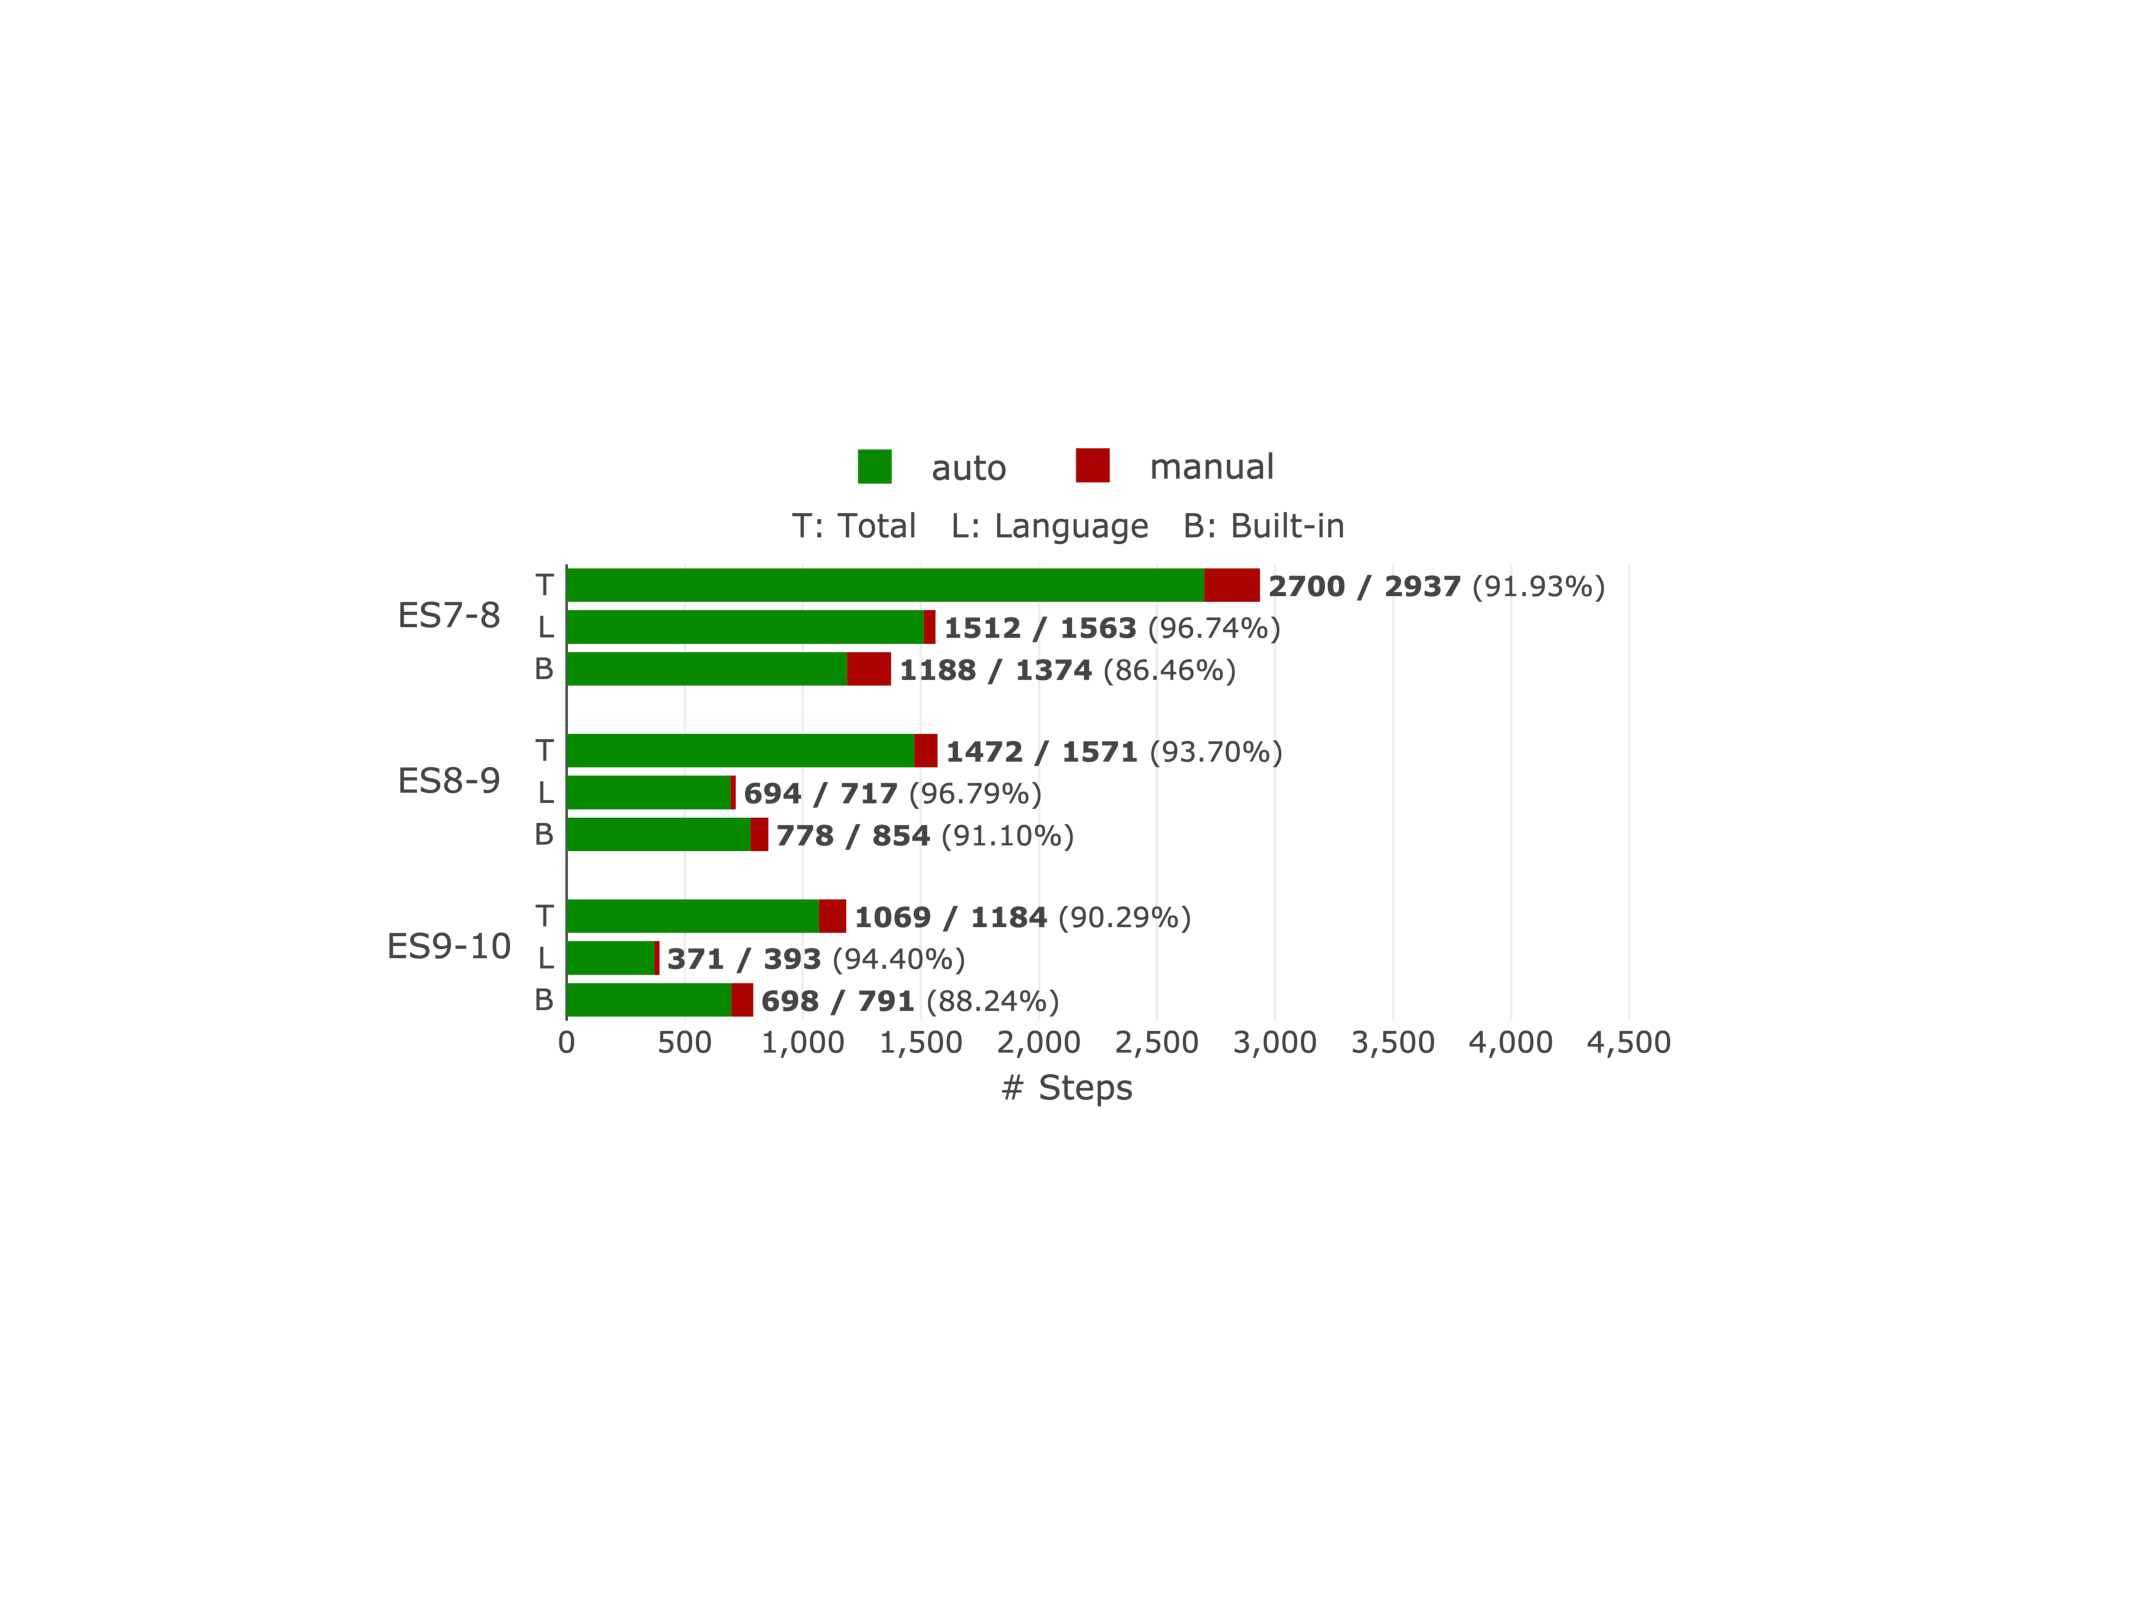
\includegraphics[width=\textwidth]{img/sem-diff.pdf}
    \caption{Results for differences between adjacent versions}
    \label{fig:semantics-all-version-diff}
  \end{subfigure}
  \caption{Number of abstract algorithm steps in specifications, from which
\( \tool \) generated the JavaScript semantics}
  \label{fig:all-version}
\vspace*{-1em}
\end{figure}

For semantics, Figure~\ref{fig:all-version} shows that \( \tool \) automatically
compile algorithm steps to the corresponding \( \ires \) instructions with
\inred{91.60\%} success rate on average for existing specifications, and
\inred{90.43\%} for updates.  ECMAScript abstract algorithms describe not only
core language semantics but also other helper functions of built-in libraries.
Built-in libraries written in more diverse styles in describing their own
specific functionalities.  Thus, built-in libraries have lower success rates
(\inred{86.98\%} for specifications and \inred{86.09\%} for updates) than core
language semantics (\inred{95.35\%} for specifications and \inred{95.25\%} for
updates).

This results show that \( \tool \) effectively reduces the efforts to
extract the syntax and semantics of JavaScript not only for developing
them from scratch, but also for updating existing ones.


\subsection{Check with Tests}\label{sec:check-with-tests}

To define the \textit{first IR-based formal semantics of modern JavaScript}, we
completed missing parts of the AST-IR translator for ES10.  Among \inred{9,674}
steps in ES10, \inred{8,901} steps are automatically compiled via
\textsf{Algorithm Compiler}.  Among the remaining \inred{773} steps, we manually
implemented all remaining language semantics (\inred{221} steps) and essential
parts of built-in libraries (\inred{XX} steps out of \inred{552}) in \inred{XX}
days.  Moreover, we manually implemented the \textsf{Global Setting} as described
in Section~\ref{sec:compiler-impl} for the core language features.  However, we
do not support several minor language features that do not affect the overall
JavaScript semantics critically: non-strict mode codes, modules, early errors
before actual executions, and inessential built-in objects.

Thanks to the executability of our extracted formal semantics, we checked the
semantics with Test262, the official conformance test suite provided by TC39.
We fixed version of Test262 as of February 28, 2019 because the ES10 was
branched out with the branch name es2019 in that day.  While it consists of
\inred{XX,XXX} tests, we filtered out \inred{XX,XXX} tests not applicable for
our formal semantics as shown in Table~\ref{table:test262}.  Test262 targets not
only the current official version of ECMAScript but several extensions and
in-progress features. We excluded \inred{X,XXX} tests for such cases to focus on
the semantics of ES10.  Among \inred{XX,XXX} ES10 tests, we also filtered out
\inred{X,XXX} tests using language features not supported by our semantics.

\begin{table*}[t]
  \centering
  \caption{Specification errors and wrong tests in Test262.}
  \label{table:spec-tests-errors}
  \vspace*{-0.5em}
  \small
  \begin{tabular}{|c|c|l|c|c|c|c|c|}
    \hline
    \multicolumn{1}{|c|}{\bf Name} &
    \multicolumn{1}{c|}{\bf Feature} &
    \multicolumn{1}{c|}{\bf Description} &
    \multicolumn{1}{c|}{\bf Known} &
    \multicolumn{1}{c|}{\bf Created} &
    \multicolumn{1}{c|}{\bf Resolved} &
    \multicolumn{1}{c|}{\bf Existed} &
    \multicolumn{1}{c|}{\bf \# Failed Tests} \\\hline

    es10-1 &
    Await &
    \makecell[l]{Passing wrong type of \\ the second argument for {\bf PromiseResolve}.} &
    \textsf{O} &
    2019-02-27 &
    2019-04-13 &
    45 days &
    \inred{XX} \\\hline

    es10-2 &
    IterationKind &
    \makecell[l]{Missing \code{async-iterate} case \\ in the assertion of {\bf
    ForIn/OfHeadEvaluation}.} &
    \textsf{X} &
    2018-02-16 &
    2020-03-25 &
    768 days &
    \inred{XX} \\\hline

    es10-3 &
    Completion &
    \makecell[l]{Not handling abrupt completion \\ in {\bf Evaluation} of {\it
    EqualityExpression}.} &
    \textsf{O} &
    2016-06-01 &
    2019-05-02 &
    1065 days &
    \inred{XX} \\\hline

    es10-4 &
    Function &
    \makecell[l]{No semantics of {\bf IsFunctionDefinition} \\ for
    \code{function(...)\{...\}}.} &
    \textsf{O} &
    2015-10-30 &
    2020-01-18 &
    1541 days &
    \inred{XX} \\\hline

    es10-5 &
    ForOf &
    \makecell[l]{Two semantics of {\bf VarScopedDeclarations} \\ for \code{for
    await(var x of e)\{...\}}.} &
    \textsf{O} &
    2018-02-16 &
    2019-10-11 &
    602 days &
    \inred{XX} \\\hline

    es10-6 &
    Argument &
    \makecell[l]{No semantics of {\bf ExpectedArgumentCount} \\ for the base case
    of {\it FormalParameters}.} &
    \textsf{O} &
    2016-11-02 &
    2020-02-20 &
    1205 days &
    \inred{XX} \\\hline

    es10-7 &
    String &
    \makecell[l]{Wrong use of \code{=} operator in {\bf
    StringGetOwnProperty}.} &
    \textsf{X} &
    2015-06-01 &
    \inred{2019-00-00} &
    \inred{XX} days &
    \inred{XX} \\\hline

    test-1 &
    Global &
    \makecell[l]{Testing implementation-dependent [[Prototype]] \\ of the global
    object.} &
    \textsf{X} &
    \inred{2019-00-00} &
    \inred{2019-00-00} &
    \inred{XX} days &
    10 \\\hline

    bigint-1 &
    UpdateExpression &
    \makecell[l]{Using wrong variable \code{oldvalue} instead of \\
    \code{oldValue} in {\bf Evaluation} of {\it UpdateExpression}.} &
    \textsf{X} &
    2019-09-27 &
    2020-04-23 &
    209 days &
    \inred{XX} \\\hline

    bigint-2 &
    NumberOp &
    \makecell[l]{Using {\bf ToInt32} instead of {\bf ToUint32} \\ in {\bf
    Number::unsignedRightShift}.} &
    \textsf{X} &
    2019-09-27 &
    2020-04-23 &
    209 days &
    \inred{XX} \\\hline

    bigint-3 &
    NumberOp &
    \makecell[l]{Using {\bf ToUint32} instead of {\bf ToInt32} \\ in {\bf
    NumberBitwiseOp}.} &
    \textsf{X} &
    2019-09-27 &
    2020-04-23 &
    209 days &
    \inred{XX} \\\hline

    bigint-4 &
    Number &
    \makecell[l]{Not handling BigInt values in {\bf Number} constructor.} &
    \textsf{O} &
    2019-09-27 &
    2019-11-19 &
    53 days &
    \inred{XX} \\\hline

  \end{tabular}
\end{table*}

\begin{table}[t]
  \centering
  \caption{Excluded tests in Test262}
  \label{table:test262}
  \vspace*{-0.5em}
  \small
  \begin{tabular}{lr}\toprule
    \belowrulesepcolor{gainsboro}
    \rowcolor{gainsboro} \textbf{All Test262 Tests} & \inred{\textbf{XX,XXX}}\\
    \aboverulesepcolor{gainsboro}\midrule
    Annexes & \inred{XXX}\\\hdashline
    Internationalization & \inred{XXX}\\\hdashline
    In-progress features & \inred{X,XXX}\\\midrule
    \belowrulesepcolor{gainsboro}
    \rowcolor{gainsboro} \textbf{ES10 Tests} & \inred{\textbf{XX,XXX}}\\
    \aboverulesepcolor{gainsboro}\midrule
    Non-strict modes & \inred{X,XXX}\\\hdashline
    Modules & \inred{X,XXX} \\\hdashline
    Early errors & \inred{X,XXX} \\\hdashline
    Inessential built-in objects & \inred{X,XXX} \\\midrule
    \belowrulesepcolor{gainsboro}
    \rowcolor{gainsboro} \textbf{Applicable Tests} & \inred{\textbf{XX,XXX}}\\
    \aboverulesepcolor{gainsboro}\midrule
    Passed tests & \inred{XX,XXX} \\\hdashline
    Failed tests & \inred{XXX} \\\bottomrule
  \end{tabular}
  \vspace*{-2em}
\end{table}

For \inred{XX,XXX} applicable tests, the synthesized JavaScript parser
successfully parses all tests but \inred{XXX} tests are failed to be executed
because of the different semantics between ECMAScript and official tests.  Based
on the failed tests, we found 7 specification errors in ES10 and 10 wrong tests
in Test262 as described in Table~\ref{table:spec-tests-errors}.  For example,
the specification error es10-1 is related to the JavaScript Await.  The {\bf
PromiseResolve (C, x)} algorithm creates a new Promise object using a given
constructor {\bf C} and resolved with a given value {\bf x}.  However, a
specification update added three invocations of {\bf PromiseResolve} with a list
of values for {\bf x} in February 27, 2019.  This error exists in 45 days until
April 13, 2019 and fails \inred{XX} tests for ES10 in Test262.  For other cases,
es10-2 arises because of the wrong assertion. es10-3 and es10-7 arise because
contributors misunderstood the meaning of abrupt completion and \code{=}
operator for numbers, respectively.  es10-4, es10-5, and es10-6 are
specification errors that miss or define twice specific corner cases of
semantic.  For example, es10-4 is an error that does not define the {\bf
IsFunctionDefinition} algorithm for unnamed functions such as
\code{function(){}}.  For these seven specification errors, they existed in ES10
in \inred{XXX} days on average.  Besides, two errors es10-2 and es10-7 are even
not known before we reported to TC39.

For tests in Test262, we found 10 wrong tests categorized in test-1 and they are
related to the JavaScript global object. The [[Prototype]] internal property of
the global object is fully implementation dependent thus the official tests
should not check its attributes.  However, 10 tests assumes that [[Prototype]]
of the global object is a prototype chain starts with \code{Object.prototype}.
They violate the implementation dependent semantics of ES10.  Moreover, they
existed in Test262 in \inred{XXX} days.

After resolving above specification errors in ES10, we extracted formal
semantics from the revised specification again. The revised formal semantics of
ES10 passed all \inred{XX,XXX} applicable tests in Test262.  We believe that our
tool can assist to check and find bugs in ECMAScript by generating executable
formal semantics and executing it with tests in Test262.


\subsection{Forward Compatibility}

We show the forward compatibility of \( \tool \) by applying it to the proposals
that are ready for inclusion in the next ECMAScript (ES11, 2020). Because
ECMAScript administered as an open-source project, various proposals for new
language features are available with their own specification changes and tests.
A separate repository~\cite{proposals} maintains such proposals with six
different stages: Stage 0 to Stage 3, Finished, and Inactive.  Each proposal
starts with Stage 0, and the TC39 committee regularly examines Stage 3 proposals
to decide their next stages.  If a proposal is confirmed, the committee changes
its stage to Finished and integrates it into the next version of ECMAScript.
Otherwise, the committee changes its stage to Inactive.  Among them, we applied
\( \tool \) to all Finished proposals decided to be included in ES11.

\begin{table}[t]
  \centering
  \caption{Evaluation result of \( \tool \) for Finished stage proposals that
  will be included in ES11.}
  \label{table:spec-prop-result}
  \vspace*{-0.5em}
  \small
  \begin{tabular}{c?r|r?r?r}
    \hline
    \multicolumn{1}{c?}{\multirow{2}{*}{\bf Name}} &
    \multicolumn{2}{c?}{\bf \( \Delta \) \# Prod.} &
    \multicolumn{1}{c?}{\multirow{2}{*}{\bf \( \Delta \) \# Steps}} &
    \multicolumn{1}{c}{\multirow{2}{*}{\bf \# Tests}} \\\cline{2-3}

    &
    \multicolumn{1}{c|}{\bf Lex.} &
    \multicolumn{1}{c?}{\bf Syn.} &
    &\\\hline\hline

    \code{matchAll} of \code{String} &
    \inred{X} &
    \inred{X} &
    9/9 &
    5/5\\\hline

    \code{import()} &
    \inred{X} &
    \inred{X} &
    \inred{X/X} &
    \inred{X/X}\\\hline

    \code{BigInt} &
    \inred{X} &
    \inred{X} &
    258/323 &
    \inred{207}/207\\\hline

    \code{Promise.allSettled} &
    \inred{X} &
    \inred{X} &
    79/85 &
    50/50\\\hline

    \code{globalThis} &
    \inred{X} &
    \inred{X} &
    1/1 &
    1/1\\\hline

    \code{for-in} mechanics &
    \inred{X} &
    \inred{X} &
    \inred{X/X} &
    \inred{X/X}\\\hline

    Optional Chaining &
    \inred{X} &
    \inred{X} &
    72/74 &
    19/19\\\hline

    Nullish Coalescing Op. &
    \inred{X} &
    \inred{X} &
    10/10 &
    21/21\\\hline

    \code{import.meta} &
    \inred{X} &
    \inred{X} &
    \inred{X/X} &
    \inred{X/X}\\\hline

    {\bf Total} &
    \inred{X} &
    \inred{X} &
    \inred{X/X} &
    \inred{X/X}\\\hline
  \end{tabular}
\end{table}

Table~\ref{table:spec-prop-result} shows the result of applying \( \tool \) to 9
Finished proposals for ES11.  For all proposals, \inred{XX} lexical and
\inred{XX} syntactic productions are modified and \( \tool \) successfully
updated the changes to the synthesized JavaScript parser.  The updated parser
parses all applicable tests for all proposals.  For abstract algorithms,
\inred{XXX} steps out of \inred{XXX} steps are automatically converted to the
corresponding \( \ires \) instructions by the algorithm compiler without
changing of the compile rules.  Thus, our tool has \inred{XX.XX\%} success rate
on average for future proposals.  Similar with
Section~\ref{sec:check-with-tests}, we manually implemented missing part of the
AST-IR translator for each Finished proposal and checked each extracted
semantics with official tests.  Each of them passed all applicable tests except
the semantics for \code{BigInt} proposal.  It fails \inred{XX} tests out of 207
applicable tests.

Based on the failed tests, we found three undiscovered specification errors
(bigint-1, bigint-2, and bigint-3), and one reported error (bigint-4) in the
BigInt proposal as described in Table~\ref{table:spec-tests-errors}.  All of
them were confirmed by TC39 and will be fixed in the next release.  The BigInt
proposal added a new type of primitives BigInt and unified the type with
original Number type to Numeric types.  Thus, it not only added new
algorithms for BigInt but also modified all existing algorithms related to
number values.  The error bigint-1 is just a simple misuse of the variable
\code{oldValue} in {\bf Evaluation} of {\it UpdateExpression}. bigint-2 and
bigint-3 break the backward compatibility because of the incorrectly mixed uses
of {\bf ToInt32} and {\bf ToUint32} algorithms in unsigned right shift operators
and bitwise operators, respectively. The last one bigint-4 arises because the
Number constructor does not consider BigInt primitives.  On average, ECMAScript
included these four specification errors in \inred{XXX} days.

After fixing all specification errors, we extracted the semantics for the BigInt
proposal again.  The updated semantics passed all 207 applicable tests.  Thus,
\( \tool \) also correctly extract IR-based semantics from future proposals.

\section{Related Work}\label{sec:related}

Type analysis of JavaScript specifications has three related topics:
JavaScript tools, mechanized specification extraction, and specification-based testing.

\paragraph{JavaScript Tools}
ECMAScript is the standard language specification for JavaScript maintained by
TC39.  In late 2014, the committee announced
its plan to release ECMAScript annually and adopt the open development process
to quickly adapt to evolving development environments.  Various JavaScript engines such
as Google V8~\cite{v8}, GraalJS~\cite{graaljs}, QuickJS~\cite{qjs}, and Moddable
XS~\cite{moddable} should conform to the syntax and semantics described in
annually updated ECMAScript.  Beyond JavaScript engines, diverse
research projects use JavaScript specifications.  The main research direction
has been static analyzers such as JSAI~\cite{jsai}, SAFE~\cite{safe},
TAJS~\cite{tajs}, and WALA~\cite{wala} based on the abstract interpretation
framework~\cite{ai1977, ai1992} with their own analysis techniques.
They defined abstract semantics of the JavaScript semantics described in ECMAScript to statically
analyze JavaScript programs in a finite time.
Chargu{\'e}raud et al.~\cite{jsexplain} presented JSExplain, a debugger for JavaScript, by
implementing a reference interpreter in OCaml following the algorithm steps in ECMAScript closely.
For a given JavaScript program, the debugger interactively produces execution traces
investigated in a browser, with an interface that displays the
JavaScript code and the interpreter's state.
Fragoso Santos et al.~\cite{javert} introduced JaVerT, a JavaScript verification toolchain, based
on the separation logic with an intermediate goto language JSIL.
JaVerT 2.0~\cite{javert2} extends it to support compositional symbolic execution
for JavaScript based on bi-abduction.  However, because all of them manually handle
ECMAScript with their own intermediate representations, most of them still 
target ES5.1 released in 2011 instead of the latest one.

\paragraph{Mechanized Specification Extraction}
Researchers in various application domains have extracted mechanized specifications from
specifications written in natural languages to handle the contents in the specifications automatically.
For system architectures, researchers utilized Natural
Language Processing (NLP) and Machine Learning techniques to extract formal semantics
of small-sized low-level assembly languages for x86~\cite{x86} and ARM~\cite{arm}.
For Java API functions, Zhai et al.~\cite{javadoc} presented a
technique to automatically extract models from their documentation using NLP techniques.
For the JavaScript programming language, Park et al.~\cite{jiset}
presented $\jiset$, a tool that extracts a mechanized specification from ECMAScript.
While all the previous JavaScript formal semantics~\cite{lambdajs, jscert,
kjs} were manually defined, $\jiset$ automatically extracts formal semantics directly from ECMAScript.
We utilized $\jiset$ to analyze 864 ECMAScript versions via $\tool$.

\paragraph{Specification-based Testing}
Recently, researchers have utilized specifications to test their implementations.
For network protocols, Kim et al.~\cite{basespec} proposed a novel approach named
\textsc{BaseSpec}, which extracts message structures from tables in cellular
specifications for L3 protocols to perform comparative analysis of baseband software.
Schumi and Sun~\cite{spectest} presented SpecTest, which utilized an
executable language semantics to perform fuzzing for Java and Solidity compilers.
For JavaScript, Ye et al.~\cite{comfort} presented \textsc{Comfort}, a
compiler fuzzing framework to detect JavaScript engine bugs using ECMAScript
with deep learning-based language models.
Park et al.~\cite{jest} extended $\jiset$ to $\jest$, which performs $N$+1-version differential testing
with $N$ different JavaScript engines and a reference interpreter extracted from ECMAScript.
$\jest$ detects not only engine bugs but also specification bugs in
ECMAScript using the cross-referencing oracle.  However, it requires multiple JavaScript engines and
takes dozens of hours to test a version of ECMAScript.
Instead, $\tool$ can detect specification bugs without JavaScript engines in two minutes.
Because $\tool$ uses abstract semantics while $\jest$ uses concrete semantics,
$\tool$ can quickly analyze more scope of semantics than $\jest$.

\section{Conclusion}\label{sec:conclusion}
Since an incorrect description in ECMAScript can lead to the wrong JavaScript
engine implementations, checking the correctness of ECMAScript is essential.
Since ECMAScript is annually released and developed in open process, it becomes
more labor-intensive and error-prone.  To alleviate the problem, we propose
$\tool$, a JavaScript Specification Type Analyzer using Refinement.  It is the
first tool that performs \textit{type analysis} on JavaScript specifications and
detects specification bugs using a \textit{bug detector}.  Moreover, to increase
precision of type analysis, we present \textit{condition-based refinement} for
type analysis, which prunes out infeasible abstract states using conditions of
assertions and branches.  We evaluated $\tool$ with all 864 versions in the
official ECMAScript repository for the recent three years from 2018 to 2021.
Our tool took \inred{137.3} seconds on average to perform type analysis for each
version, and detected \inred{161} type-related specification bugs with
\inred{56.5}\% precision; \inred{91} out of \inred{161} bugs are true bugs.
Among them, \inred{14} bugs are newly detected by $\tool$, and the committee
confirmed all of them.


\bibliographystyle{ACM-Reference-Format}
\bibliography{ref}

\end{document}
\endinput
